\begin{center}
  \textbf{Отчёт лабораторной работы №\envReportLabNumber}
\end{center}

\textbf{Тема}:
<<\envReportTitle>>

\begin{center}
  \textbf{Логическая модель}
\end{center}

Логическая модель изображена на рисунке~\ref{fig:logic_model}.

\begin{figure}[!h]
  \centering

  \includegraphics[width=21cm, angle=90]
  {../database/logic_model.pdf}

  \caption{Логическая модель}

  \label{fig:logic_model}
\end{figure}

\newpage

\begin{center}
  \textbf{Задание 1}
\end{center}

\textbf{Условие}:
Написать хранимую процедуру, которая осуществляет по окончании летней сессии, т.е. в период с 1 июля по 31 августа текущего года,
перевод всех студентов таблицы STUDENT базы данных STUDENTS на следующий курс,
а данные студентов, окончивших пятый курс, удаляет из базы данных.

\begin{center}
  \textbf{Решение задания 1}
\end{center}

\lstinputlisting[language=sql]{../sql/task1/1.sql}

\textbf{Результат}: выборка количества студентов в университете по курсам изображены на рисунках~\ref{fig:task1_1},
\ref{fig:task1_2}, \ref{fig:task1_3}, \ref{fig:task1_4}, \ref{fig:task1_5}, \ref{fig:task1_6}.

\begin{figure}[!h]
  \centering

  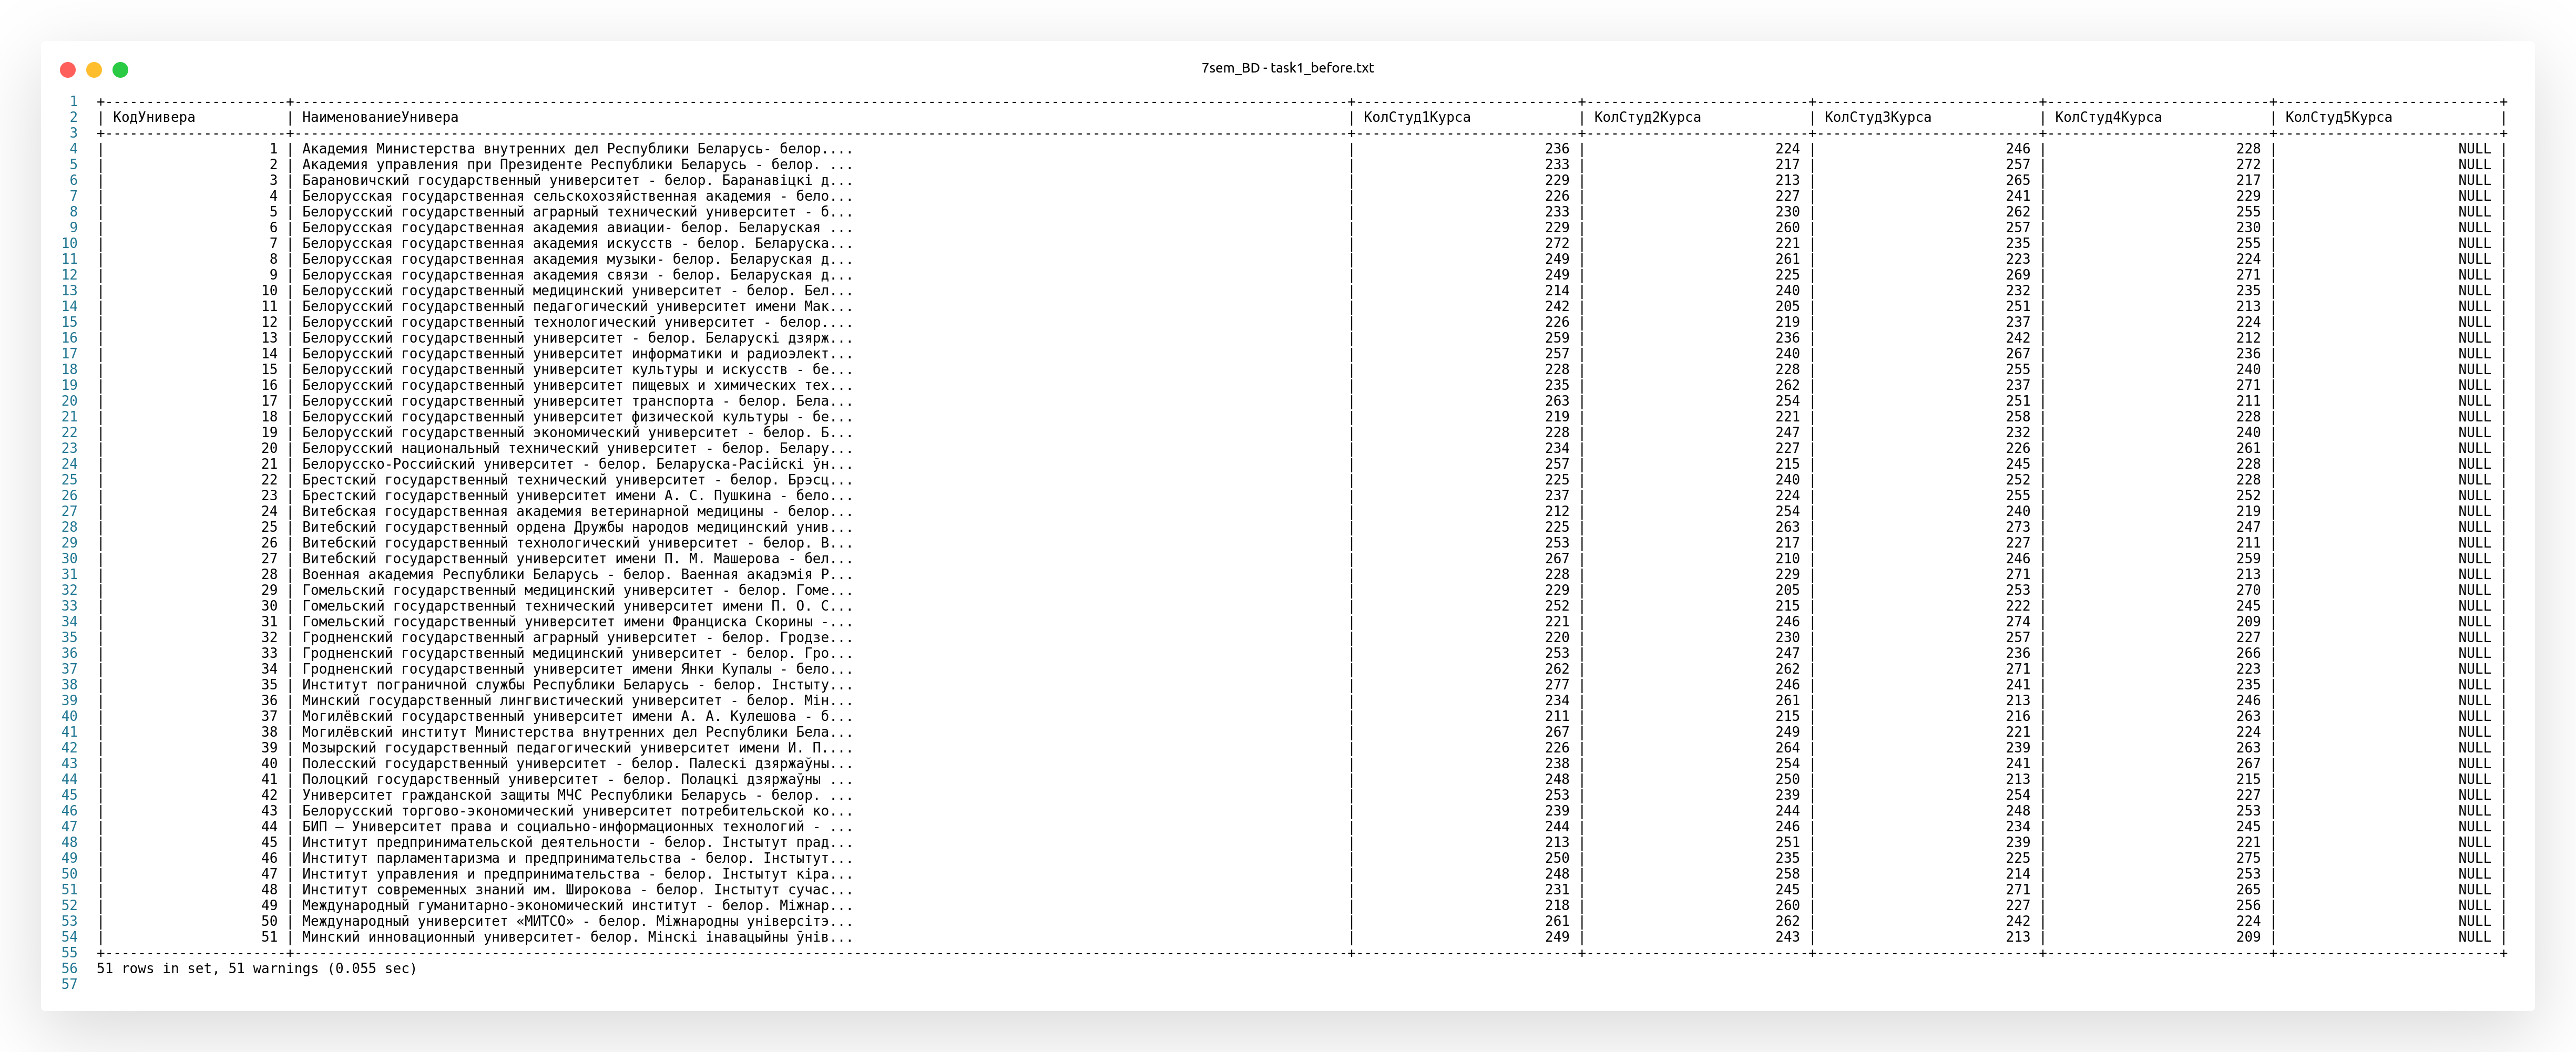
\includegraphics[width=18cm]
  {../sql/task1/task1_before.png}

  \caption{База данных студентов университетов}

  \label{fig:task1_1}
\end{figure}

\begin{figure}[!h]
  \centering

  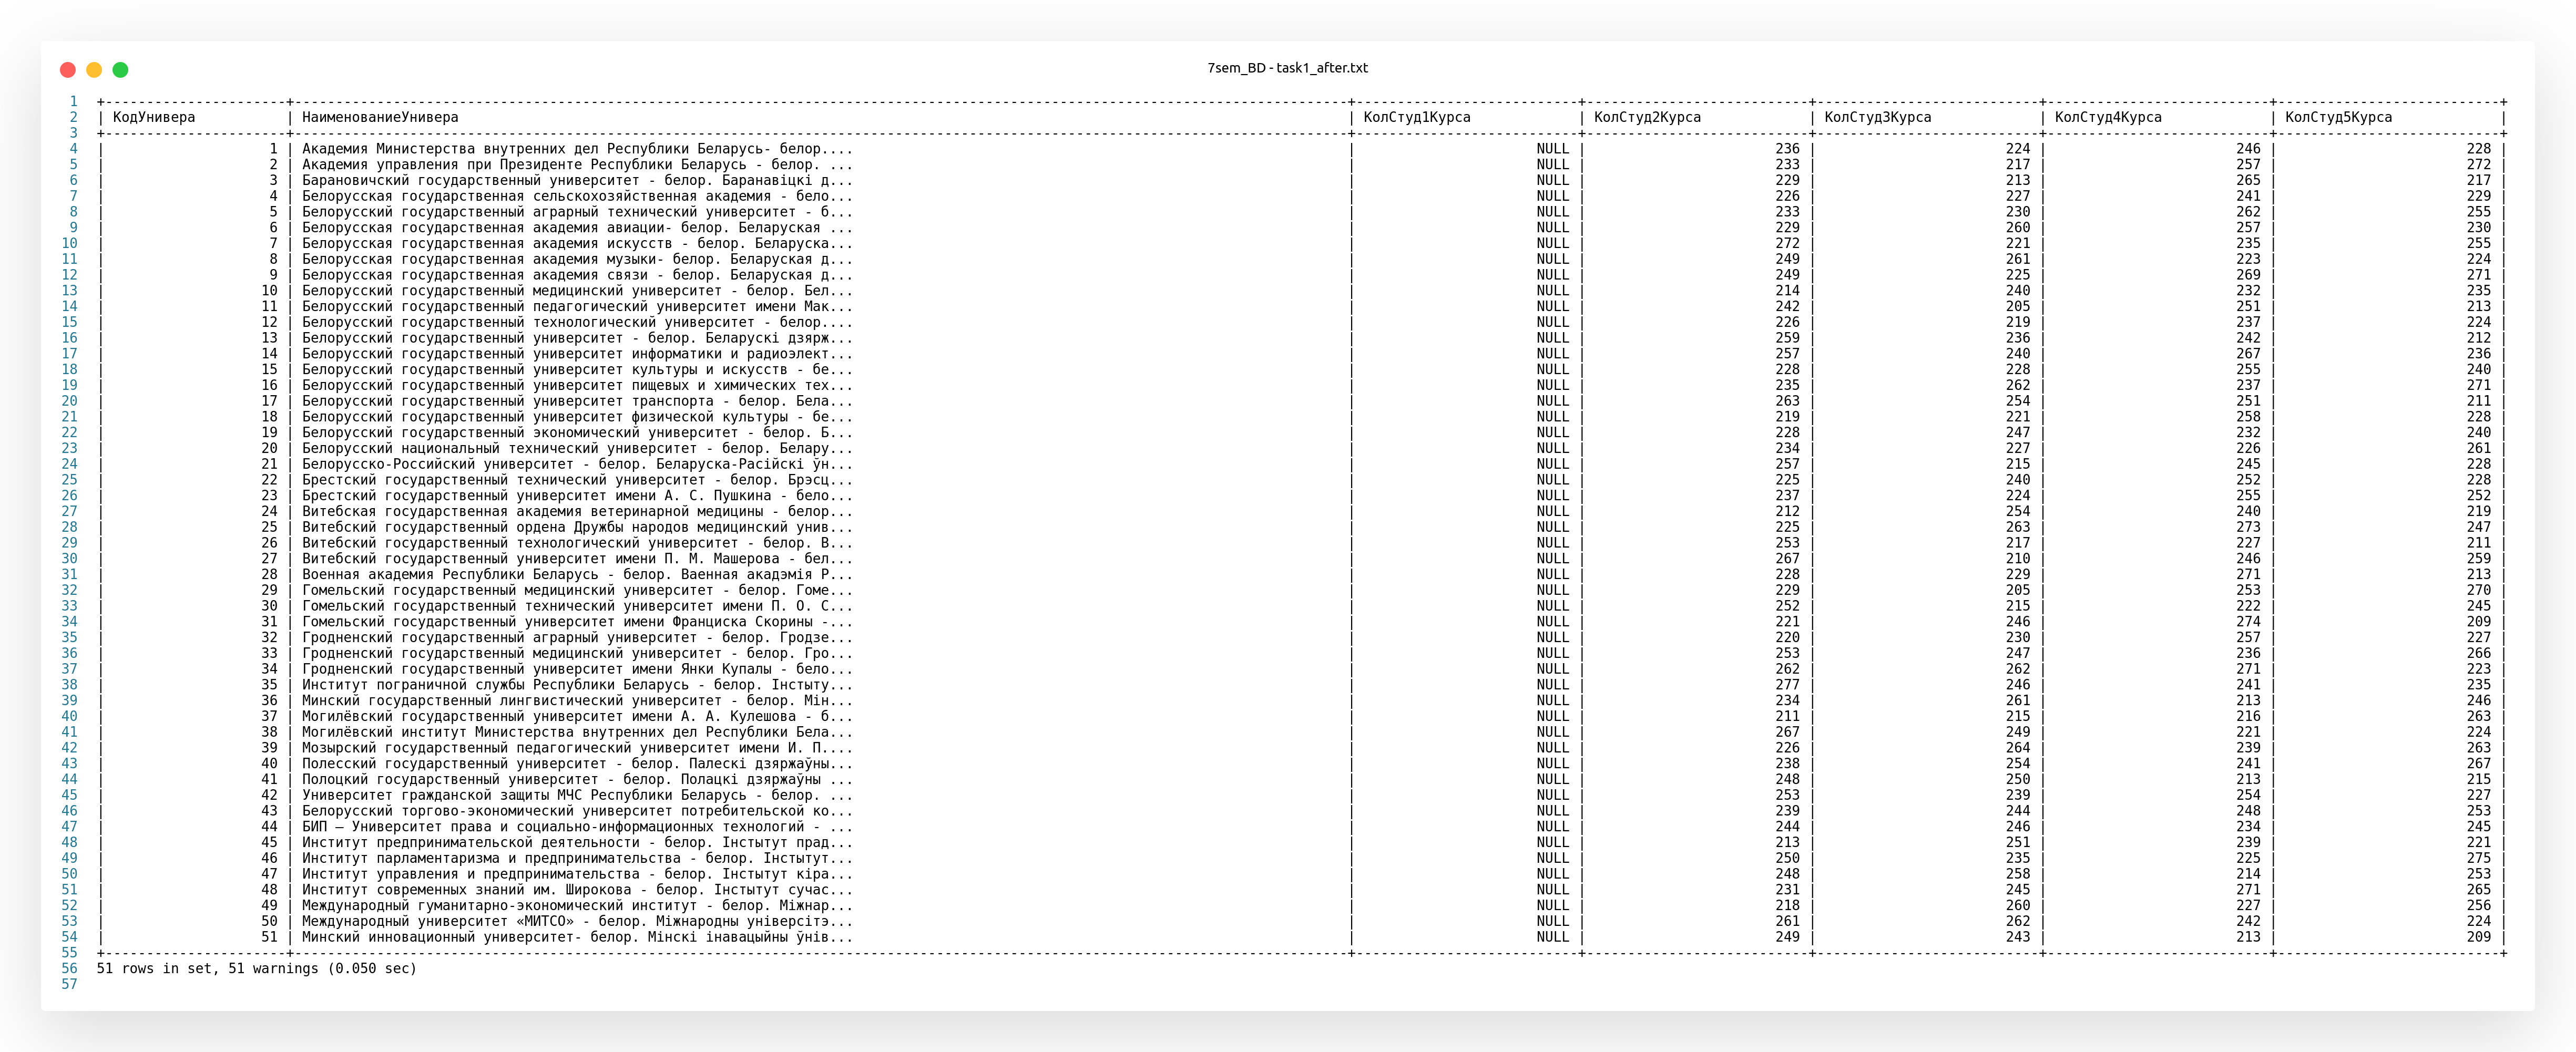
\includegraphics[width=18cm]
  {../sql/task1/task1_after.png}

  \caption{База данных после перевода студентов на следующий курс}

  \label{fig:task1_2}
\end{figure}

\begin{figure}[!h]
  \centering

  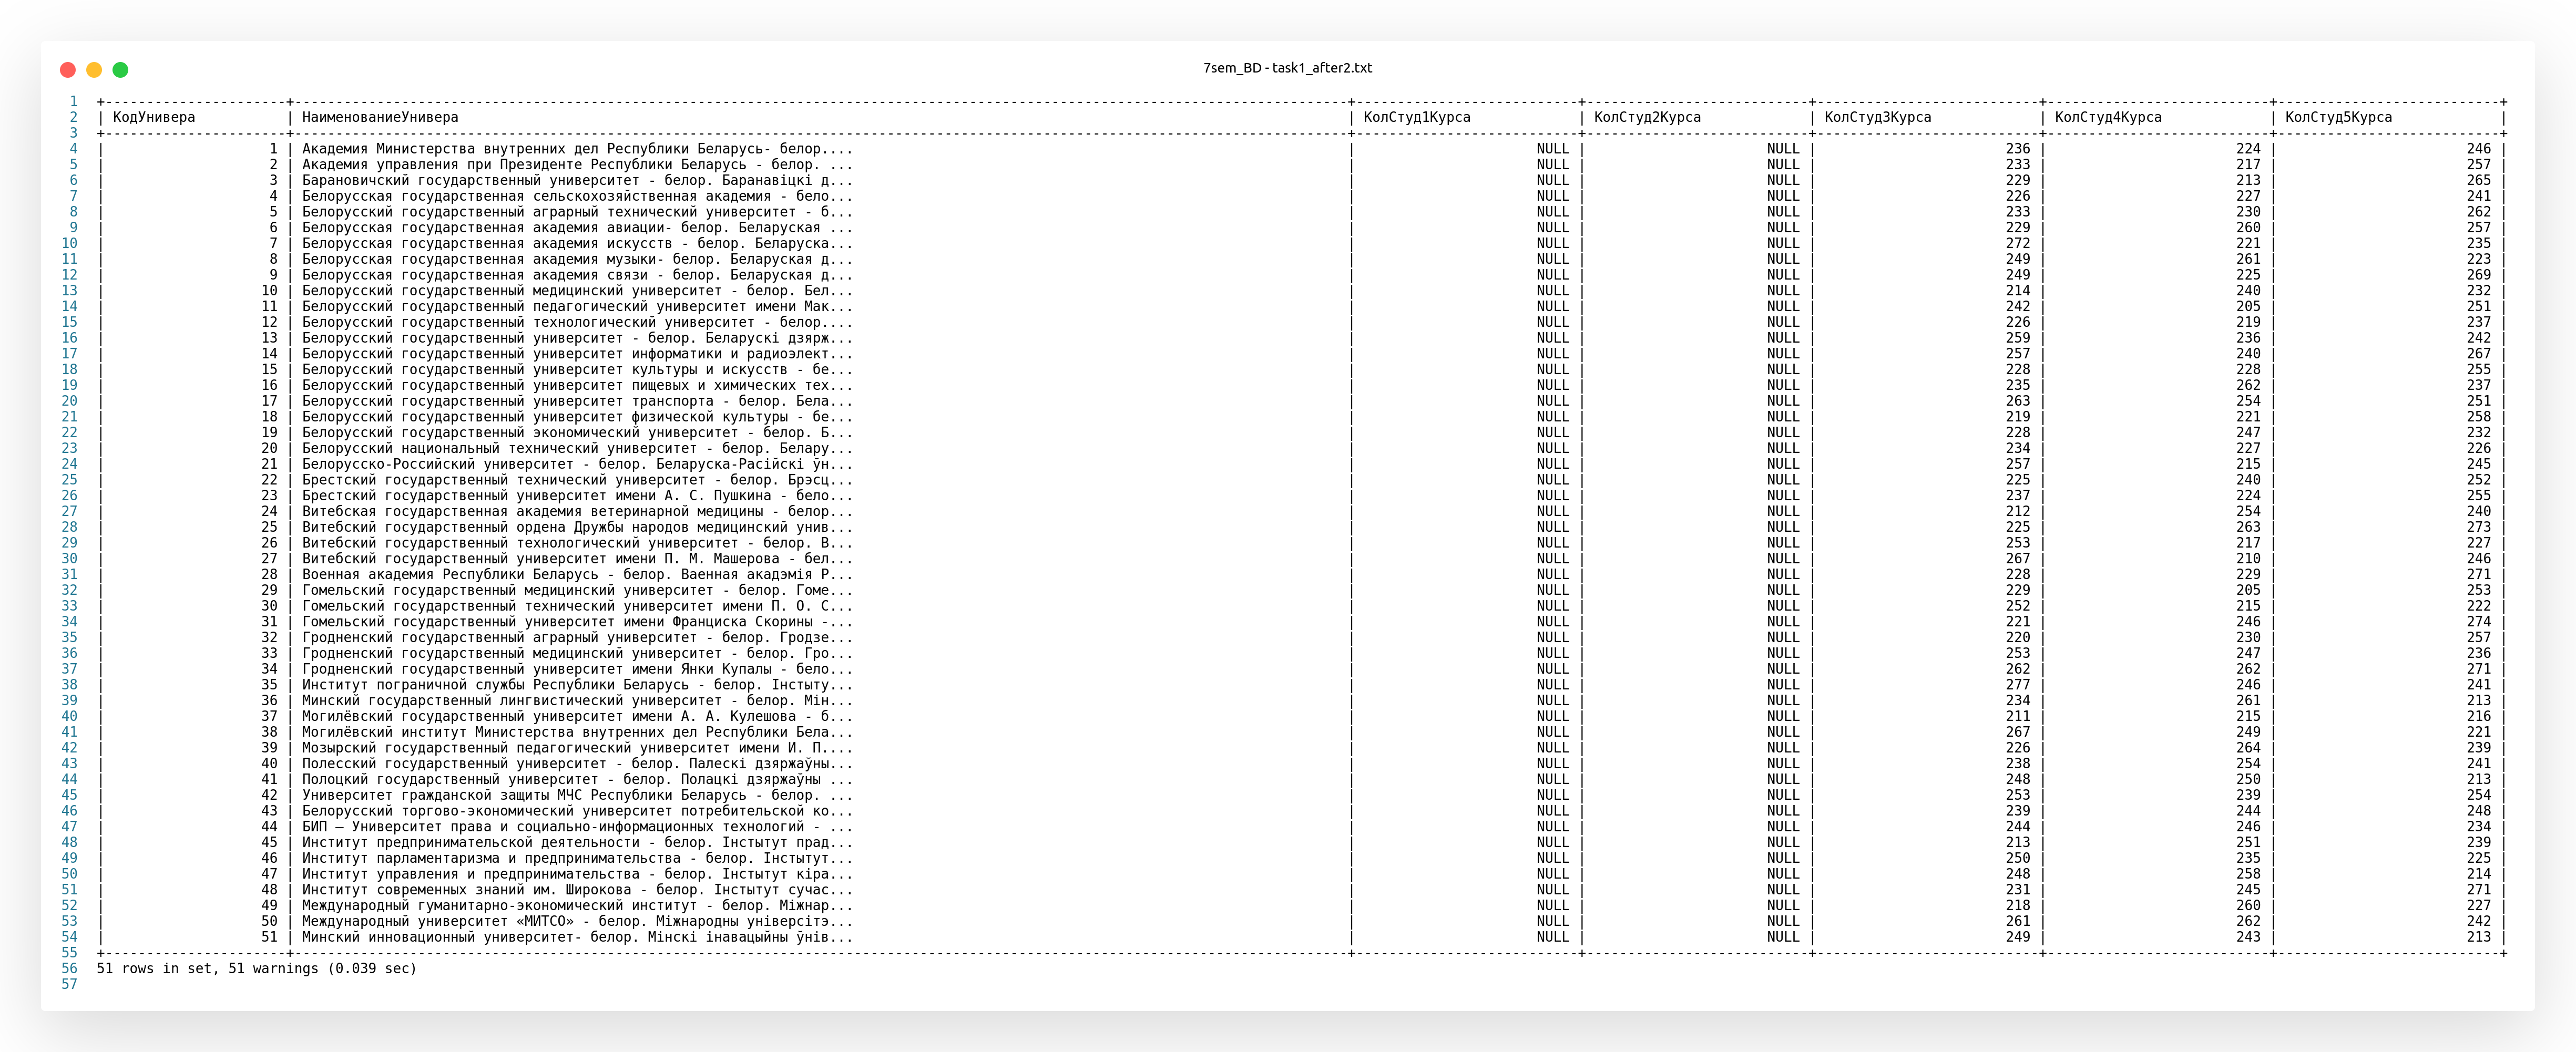
\includegraphics[width=18cm]
  {../sql/task1/task1_after2.png}

  \caption{База данных после перевода студентов на следующий курс}

  \label{fig:task1_3}
\end{figure}

\begin{figure}[!h]
  \centering

  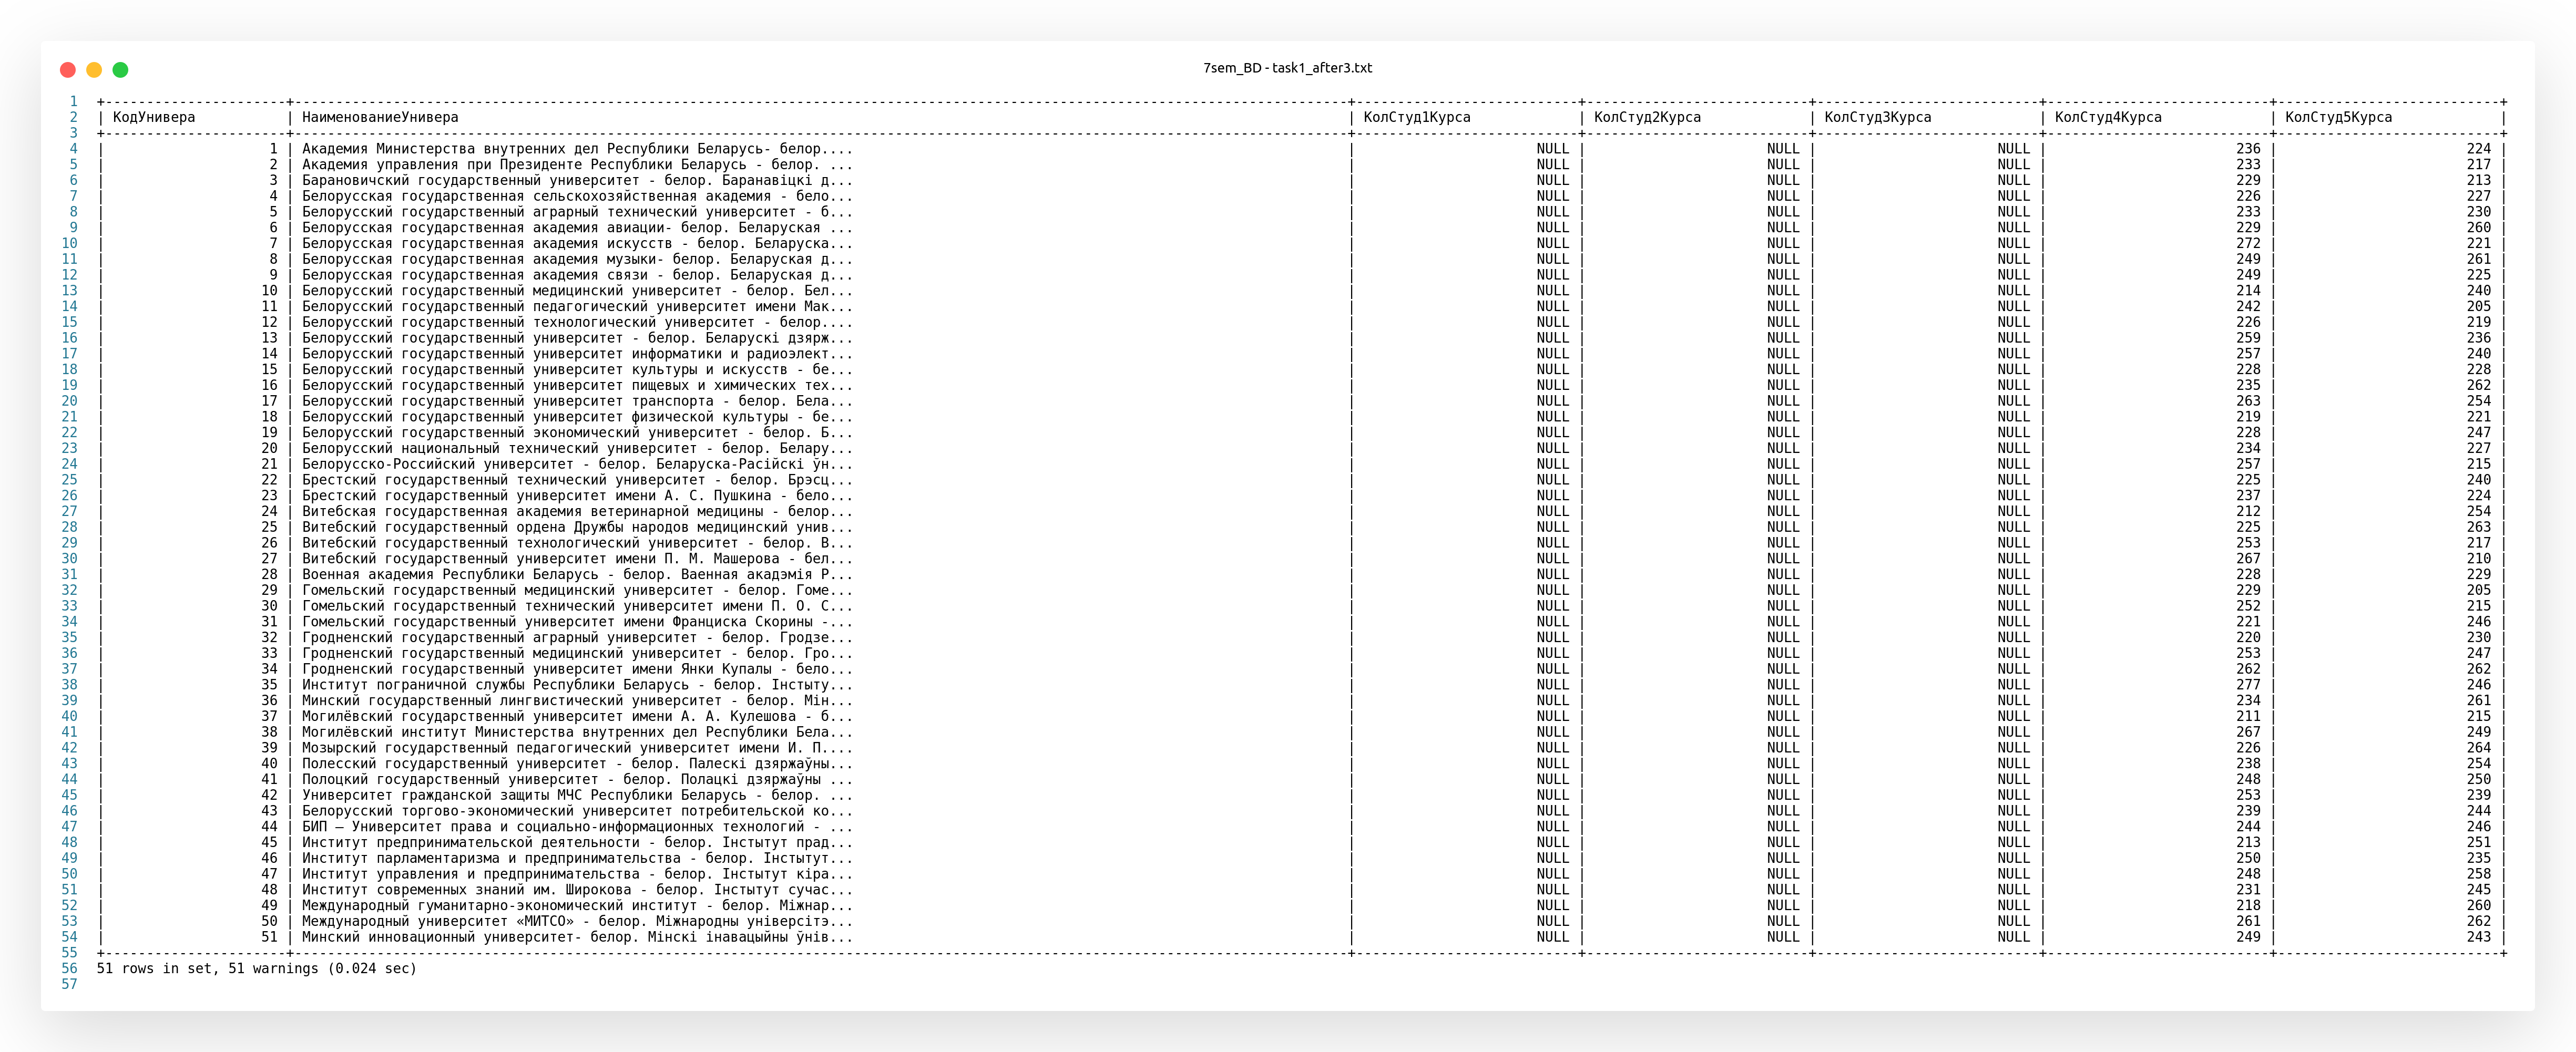
\includegraphics[width=18cm]
  {../sql/task1/task1_after3.png}

  \caption{База данных после перевода студентов на следующий курс}

  \label{fig:task1_4}
\end{figure}

\begin{figure}[!h]
  \centering

  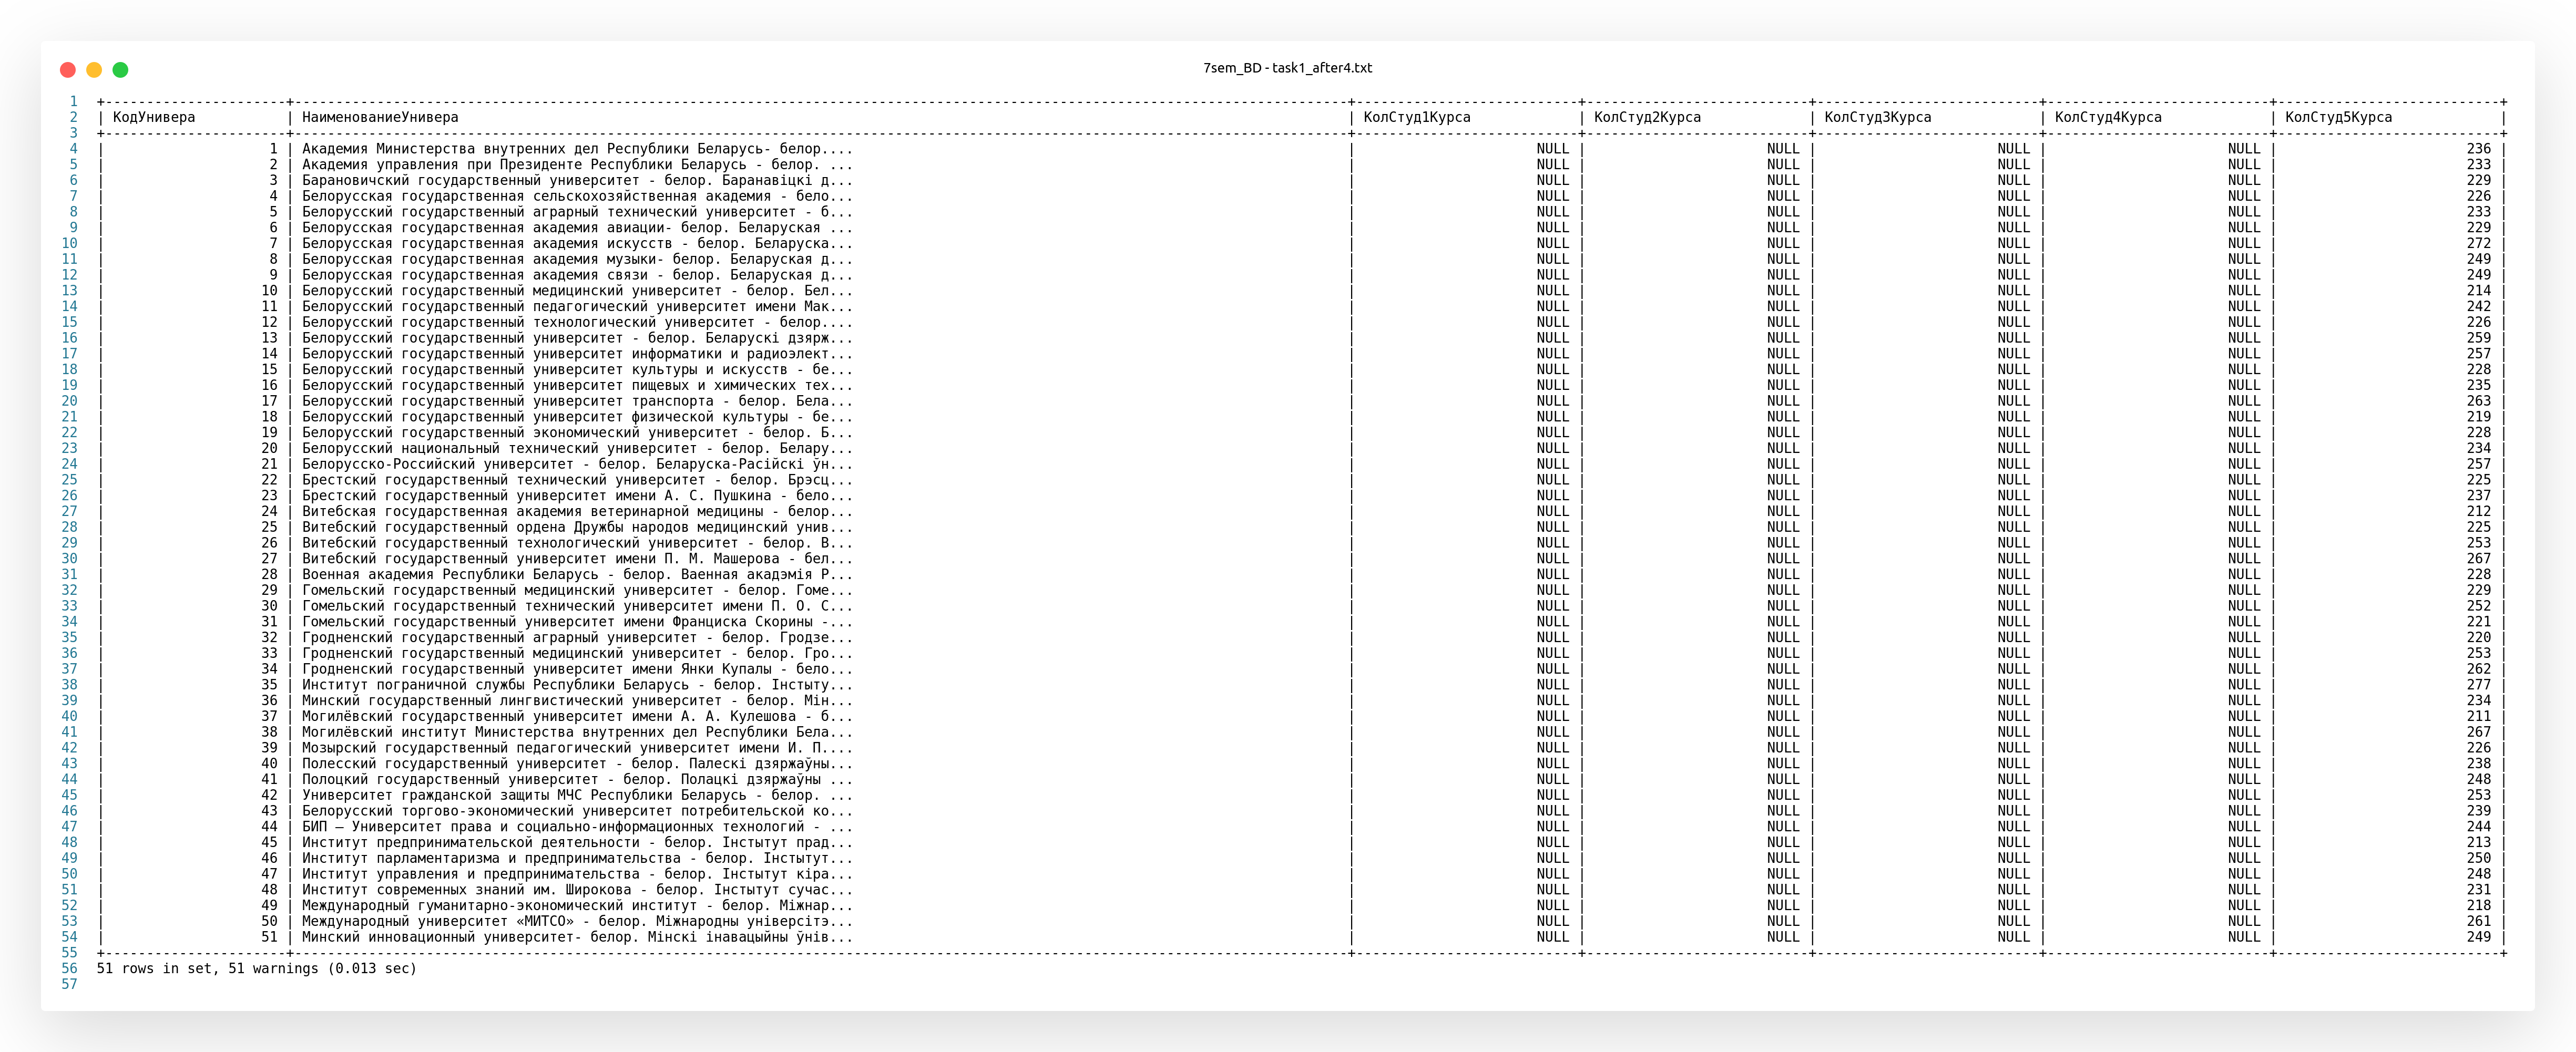
\includegraphics[width=18cm]
  {../sql/task1/task1_after4.png}

  \caption{База данных после перевода студентов на следующий курс}

  \label{fig:task1_5}
\end{figure}

\begin{figure}[!h]
  \centering

  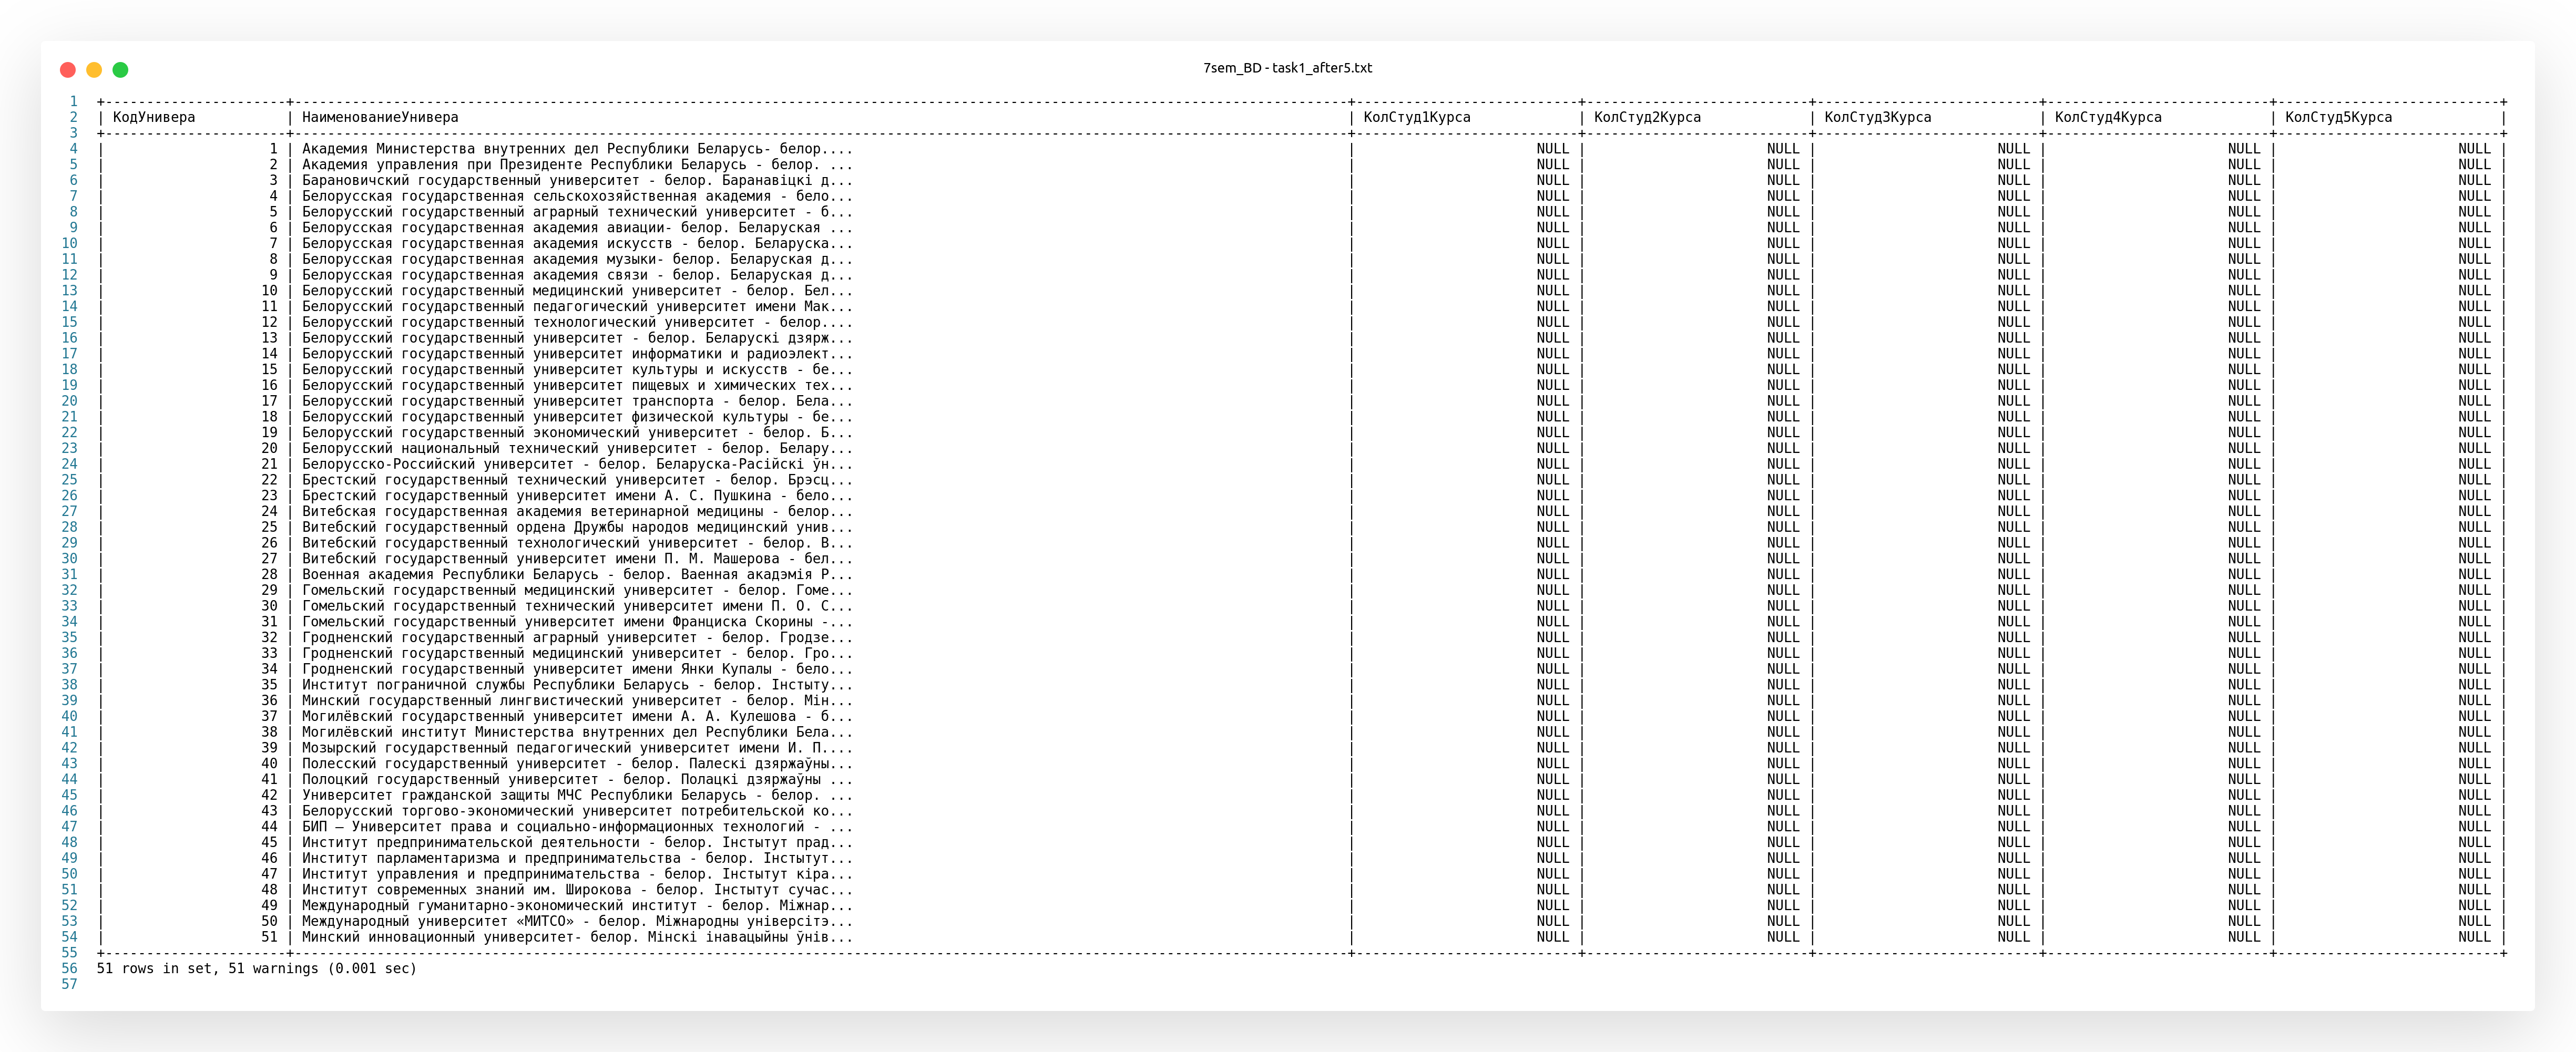
\includegraphics[width=18cm]
  {../sql/task1/task1_after5.png}

  \caption{База данных после перевода студентов на следующий курс}

  \label{fig:task1_6}
\end{figure}

\newpage

\begin{center}
  \textbf{Задание 2}
\end{center}

\textbf{Условие}:
Написать хранимую процедуру, изменяющую величину стипендии всем студентам на заданный процент по окончании сессии,
рассчитываемый по схеме:\\ $10 * (\text{Ср. балл} - 5)\%$.

\begin{center}
  \textbf{Решение задания 2}
\end{center}

\lstinputlisting[language=sql]{../sql/task2/2.sql}

\textbf{Результат}: выборка количества студентов в университете по курсам изображены на рисунках~\ref{fig:task1_1},
\ref{fig:task1_2}, \ref{fig:task1_3}, \ref{fig:task1_4}, \ref{fig:task1_5}, \ref{fig:task1_6}.

\begin{figure}[!h]
  \centering

  \begin{minipage}{0.49\textwidth}
    \centering

    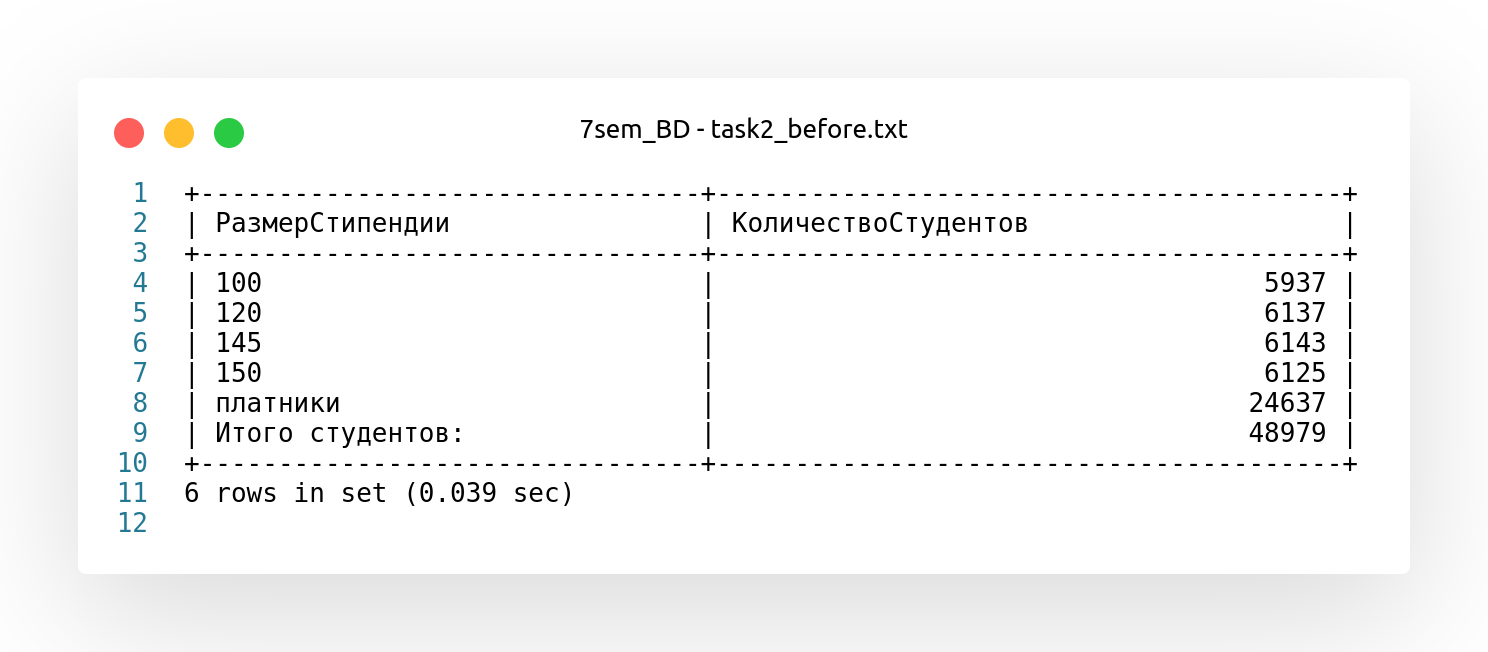
\includegraphics[width=9cm]
    {../sql/task2/task2_before.png}

    \caption{Стипендии и количество студентов}
    \label{fig:task2_1}
  \end{minipage}
  \begin{minipage}{0.49\textwidth}
    \centering

    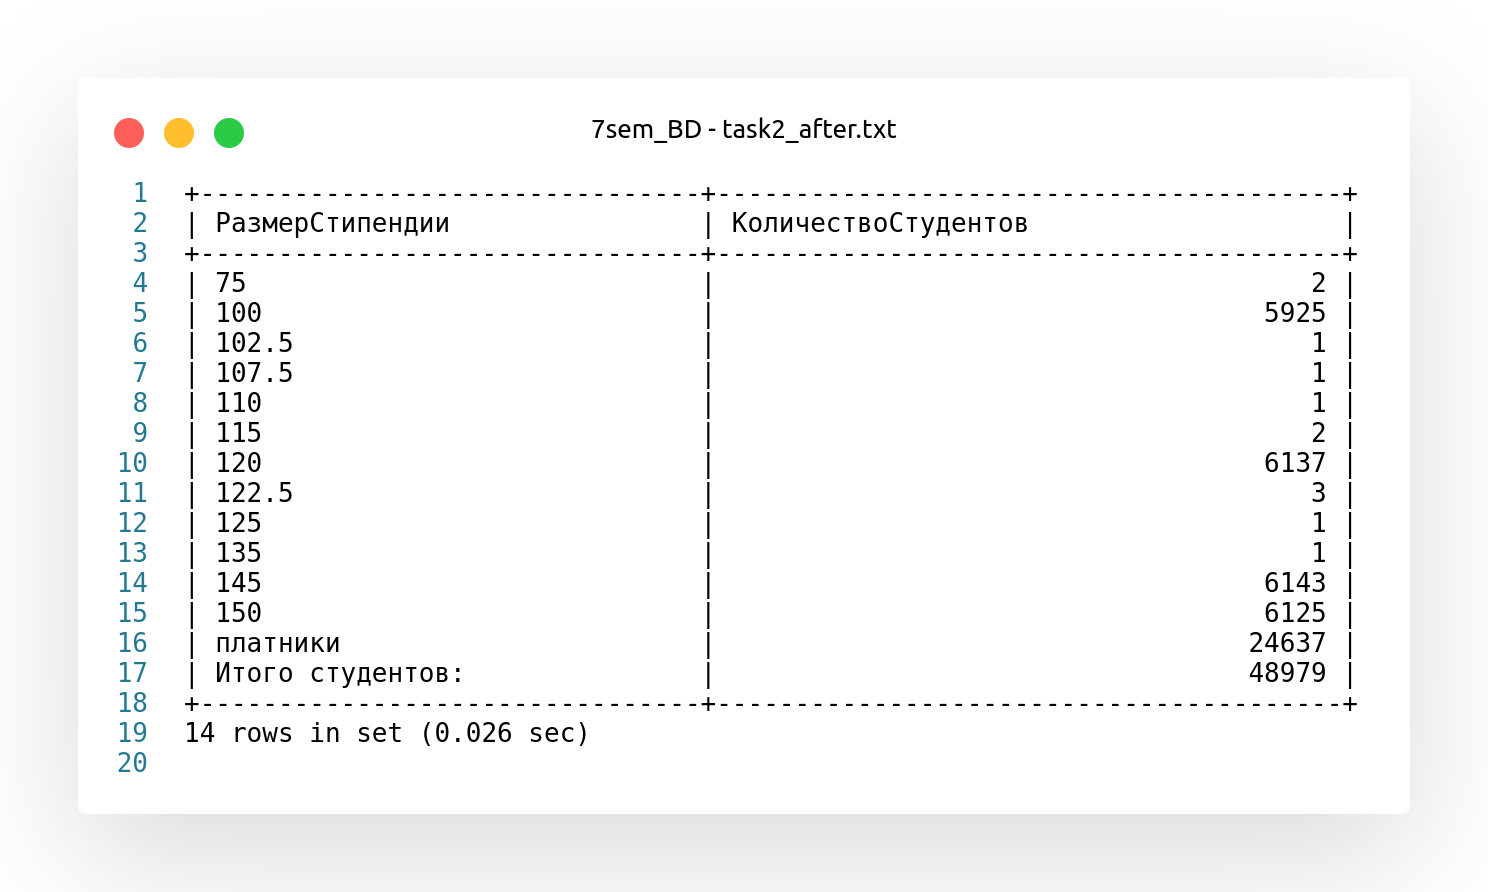
\includegraphics[width=9cm]
    {../sql/task2/task2_after.png}

    \caption{Стипендии и количество студентов после корректировки}
    \label{fig:task2_2}
  \end{minipage}
\end{figure}

\begin{center}
  \textbf{Задание 3}
\end{center}

\textbf{Условие}:
Написать хранимую процедуру, передающую по заданному ID персональную информацию о студенте
(ФИО, курс, величину стипендии, средний балл) во внешние по отношению к хранимой процедуре переменные.
Значения переменных вывести на экран.

\begin{center}
  \textbf{Решение задания 3}
\end{center}

\lstinputlisting[language=sql]{../sql/task3/3.sql}

\textbf{Результат}: значение переменных изображены на рисунках~\ref{fig:task3_1}, \ref{fig:task3_2}.

\begin{figure}[!h]
  \centering

  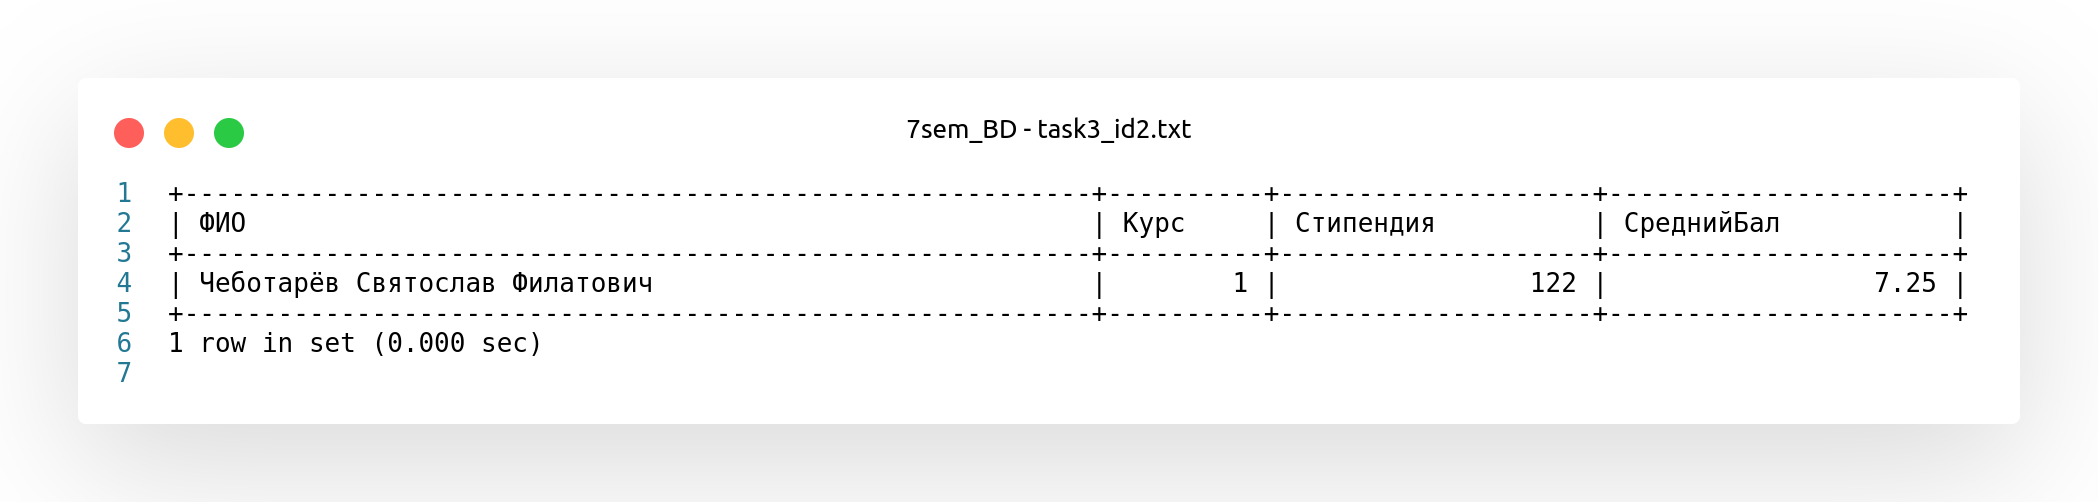
\includegraphics[width=18cm]
  {../sql/task3/task3_id2.png}

  \caption{Значение переменных для ид = 2}

  \label{fig:task3_1}
\end{figure}

\begin{figure}[!h]
  \centering

  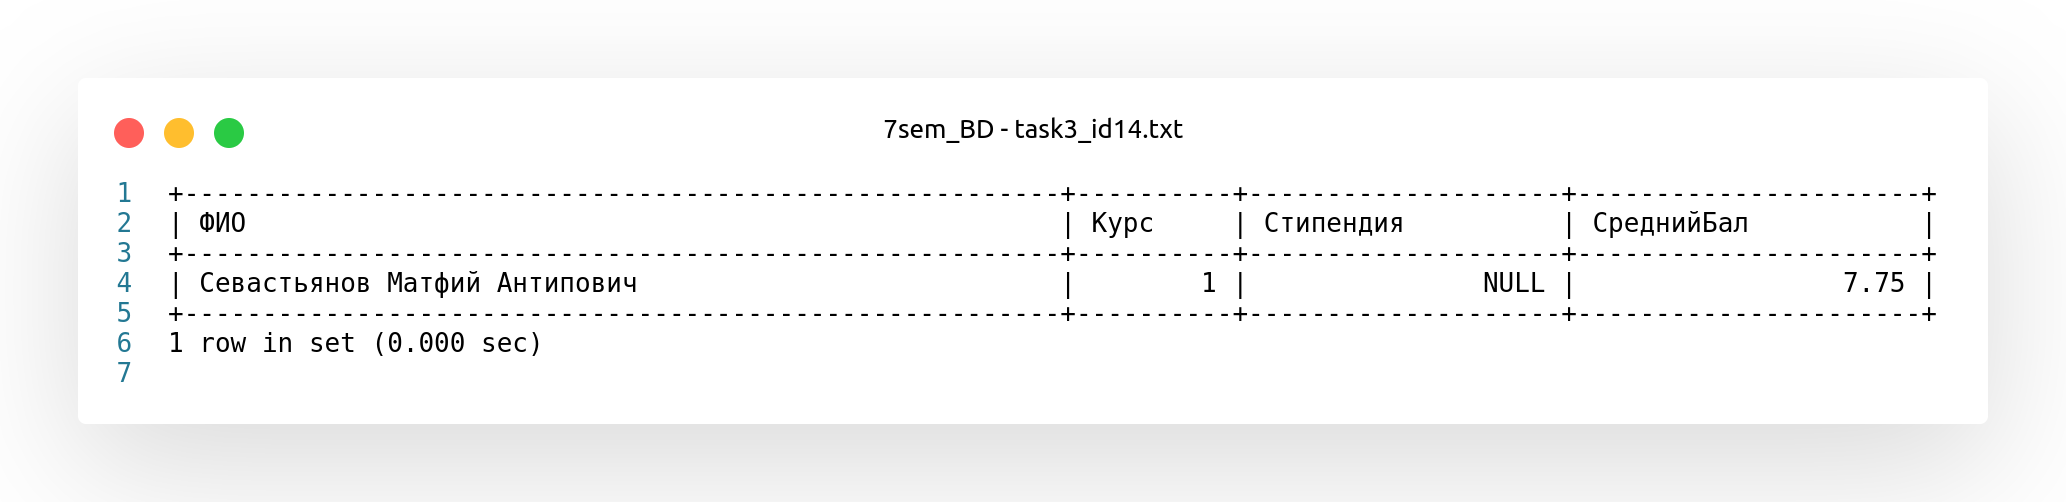
\includegraphics[width=18cm]
  {../sql/task3/task3_id14.png}

  \caption{Значение переменных для ид = 14}

  \label{fig:task3_2}
\end{figure}

\begin{center}
  \textbf{Задание 4}
\end{center}

\textbf{Условие}:
Написать хранимую процедуру, осуществляющую вставку в таблицу University новую запись cо следующим комментарием о рейтинге университета:
<<Высокий>>, если рейтинг нового университета более 7,
<<Низкий>>, если рейтинг менее 5,
<<Средний>>, если рейтинг находится в диапазоне от 5 и до 7.
При необходимости в таблицу добавить соответствующий столбец для хранения комментария.

\begin{center}
  \textbf{Решение задания 4}
\end{center}

\lstinputlisting[language=sql]{../sql/task4/4.sql}

\textbf{Результаты} изображены на рисунках~\ref{fig:task4_1},
\ref{fig:task4_2}, \ref{fig:task4_4}.

\begin{figure}[!h]
  \centering

  \begin{minipage}{0.49\textwidth}
    \centering

    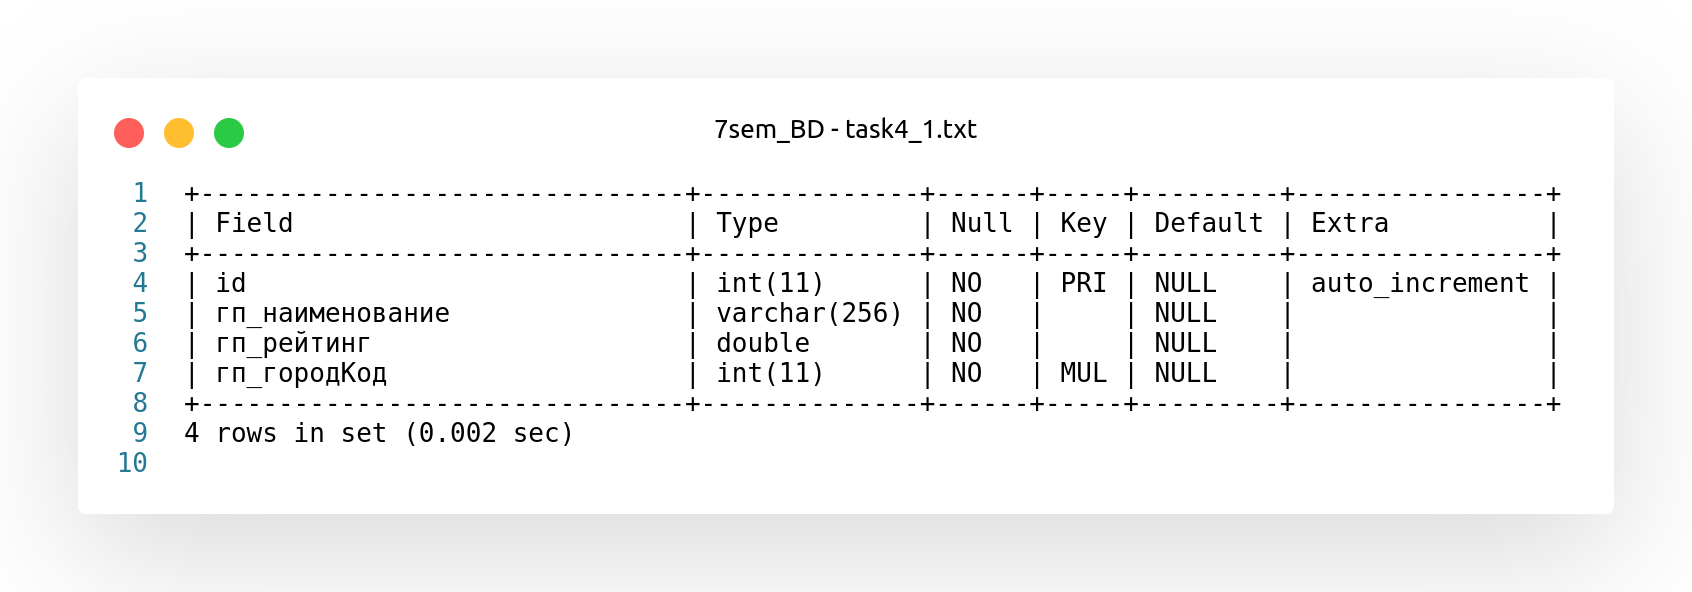
\includegraphics[width=9cm]
    {../sql/task4/task4_1.png}

    \caption{Атрибуты таблицы университетов}
    \label{fig:task4_1}
  \end{minipage}
  \begin{minipage}{0.49\textwidth}
    \centering

    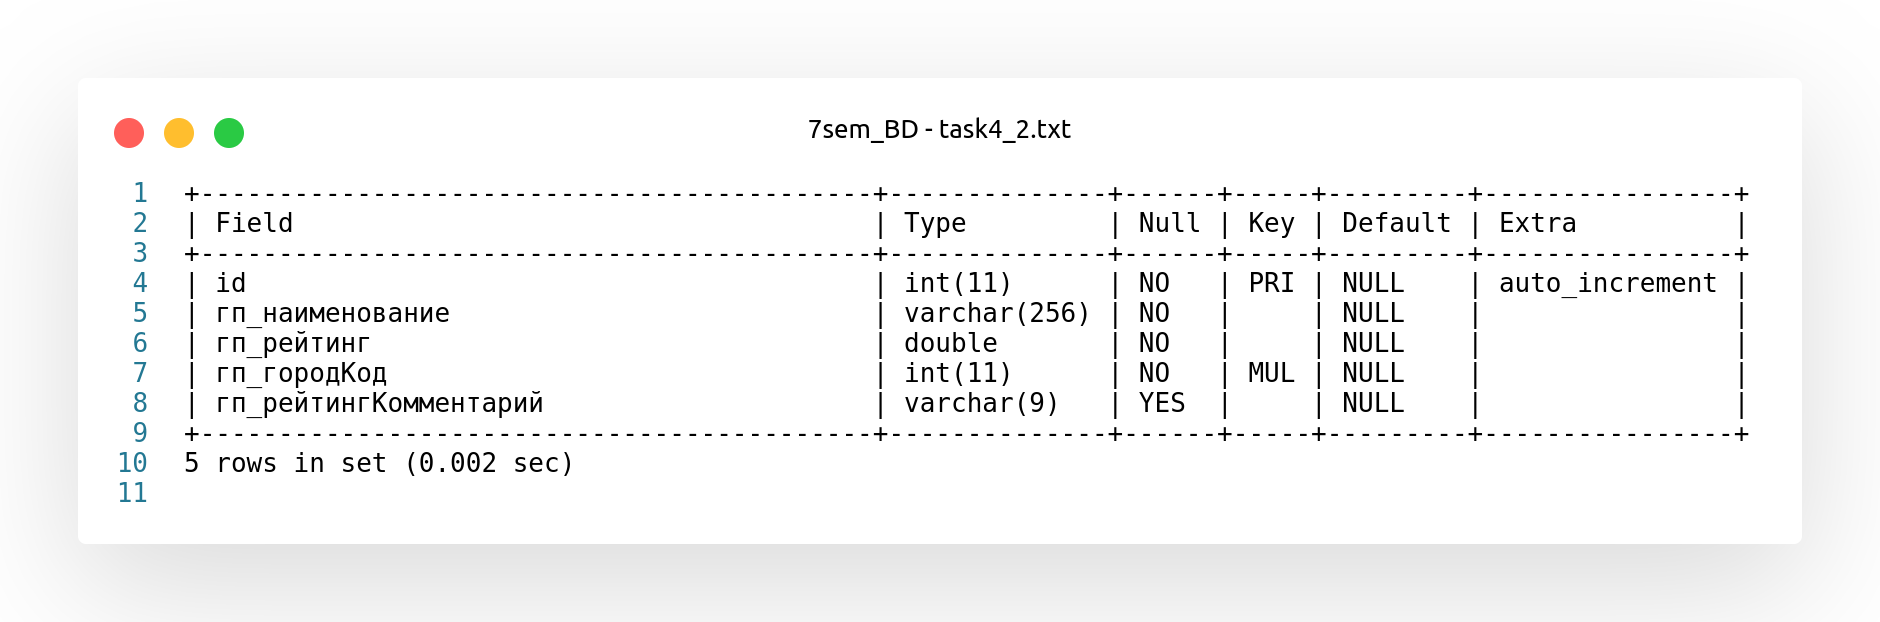
\includegraphics[width=9cm]
    {../sql/task4/task4_2.png}

    \caption{Атрибуты таблицы университетов}
    \label{fig:task4_2}
  \end{minipage}
\end{figure}

% \begin{figure}[!h]
%   \centering

%   \includegraphics[width=18cm]
%   {../sql/task4/task4_3.png}

%   \caption{Выборка университетов}

%   \label{fig:task4_3}
% \end{figure}

\begin{figure}[!h]
  \centering

  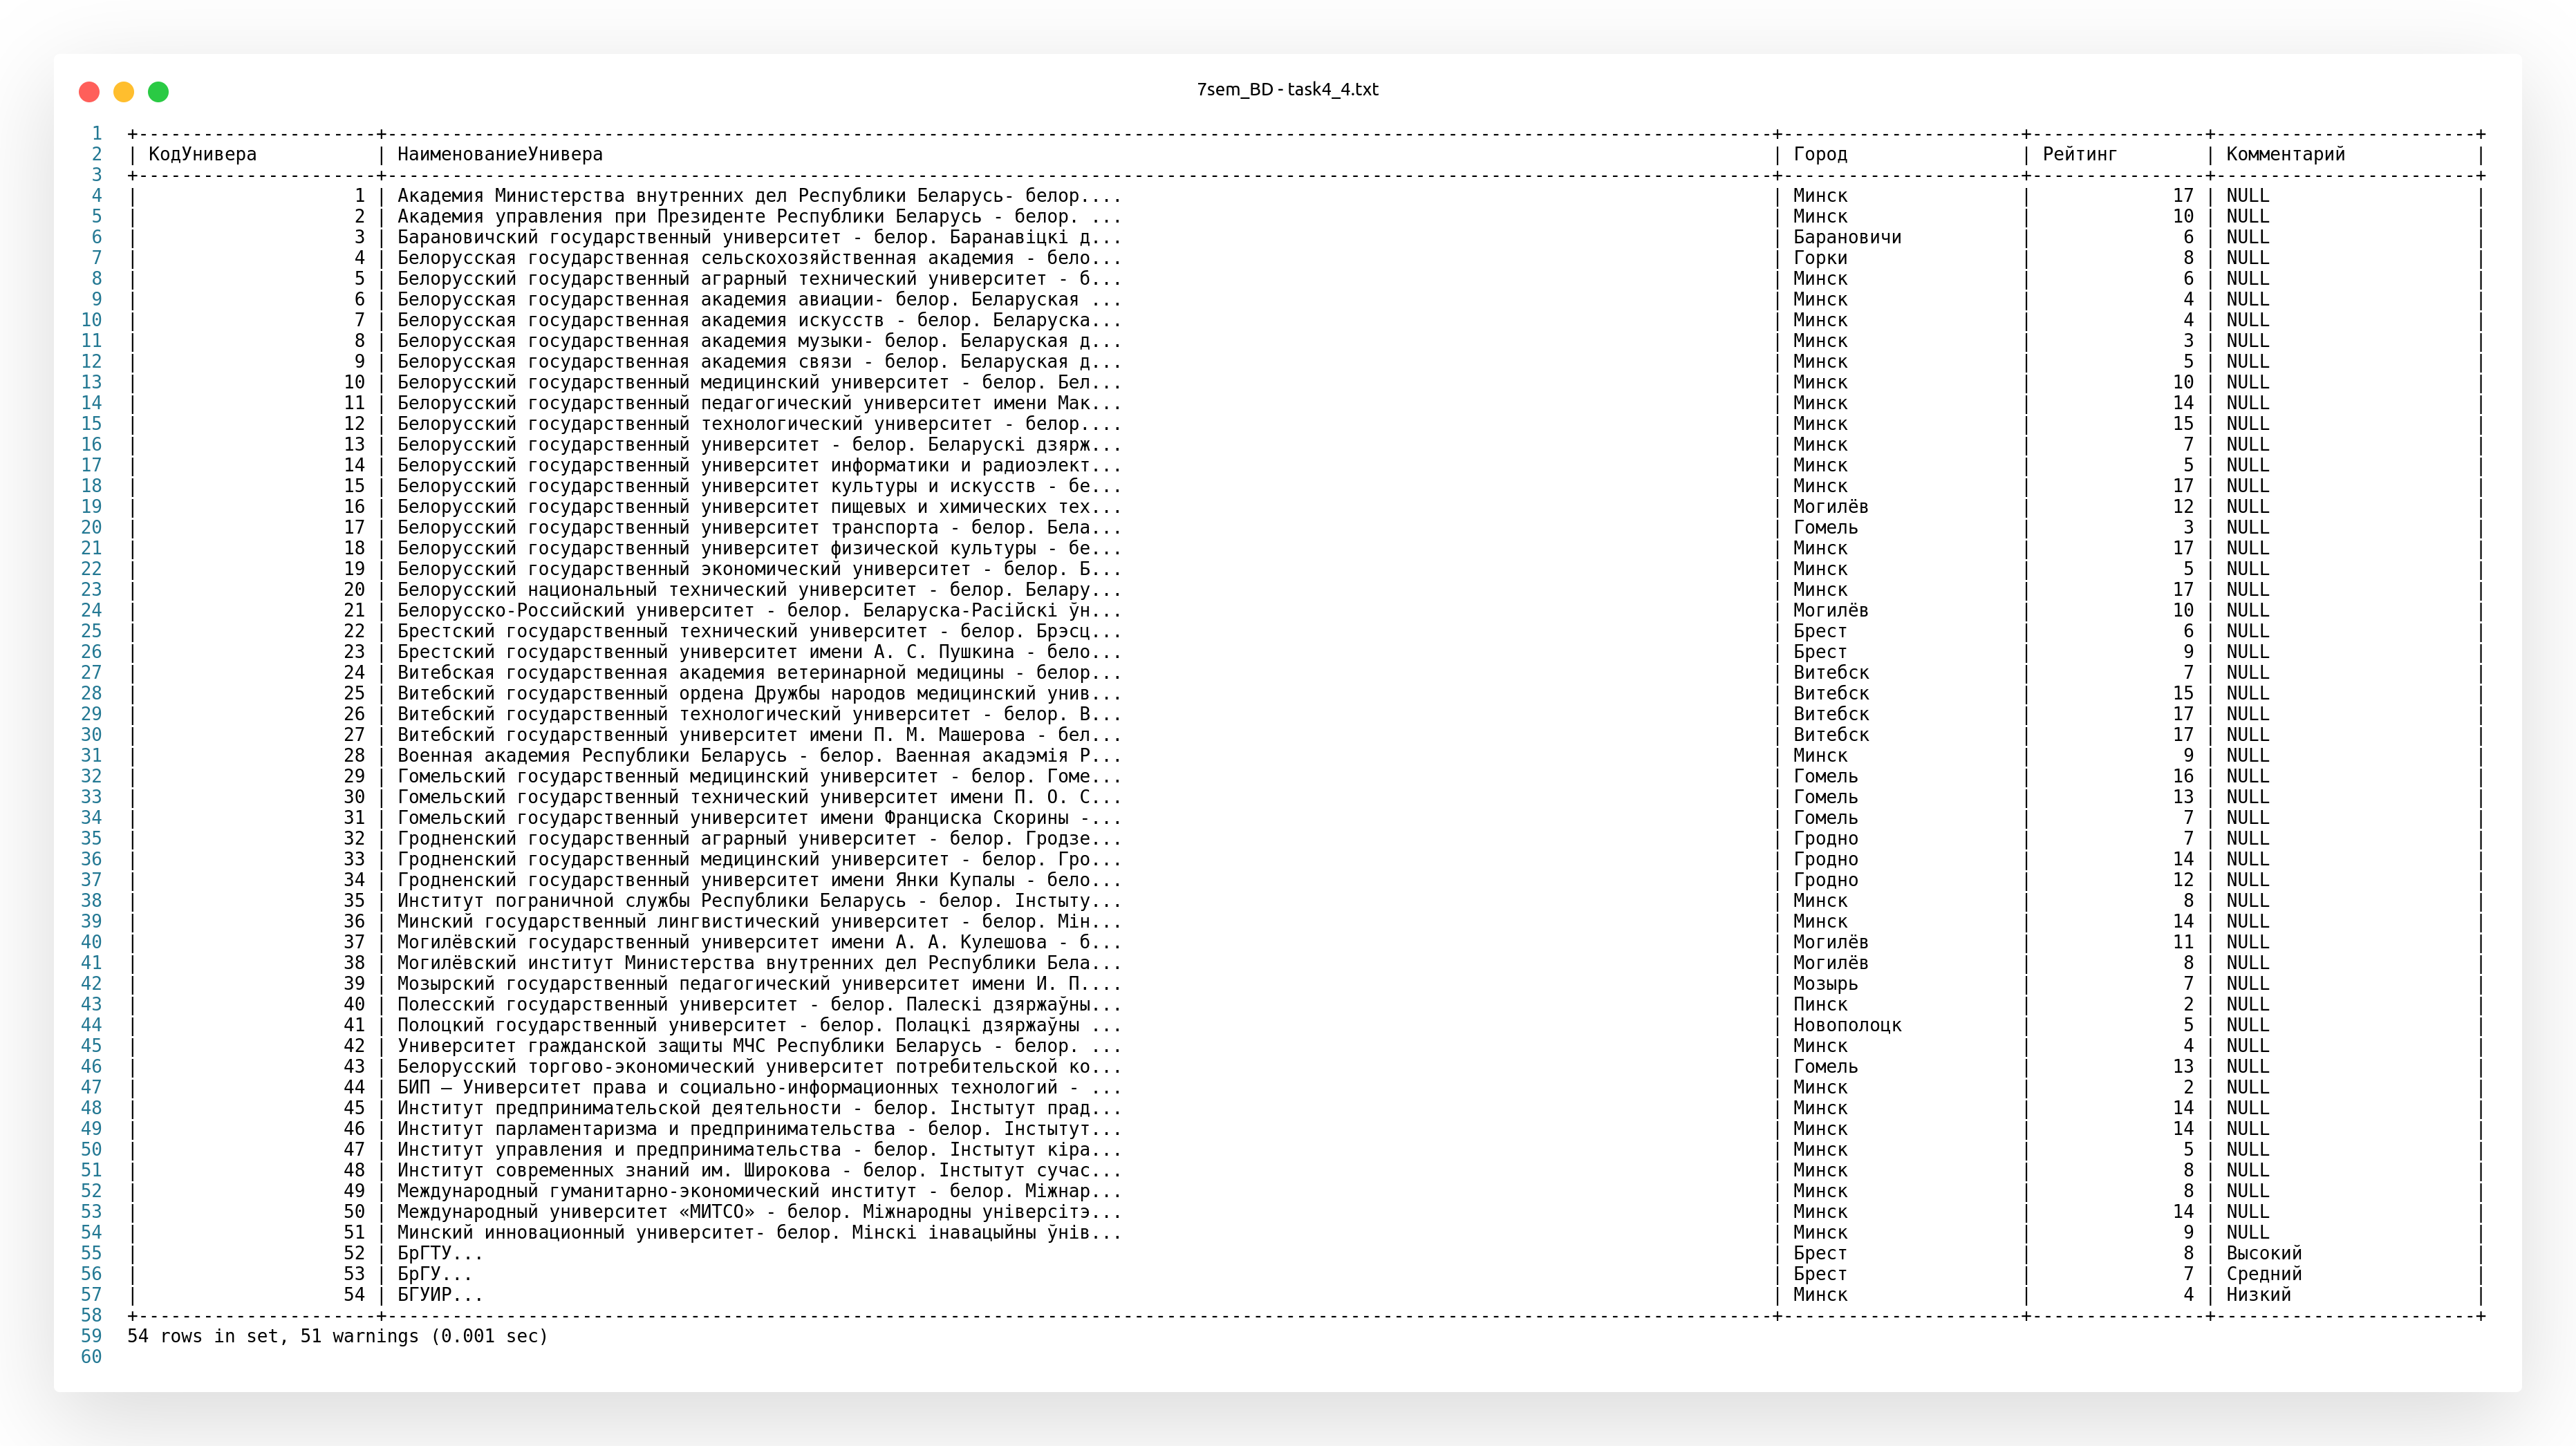
\includegraphics[width=18cm]
  {../sql/task4/task4_4.png}

  \caption{Выборка университетов}

  \label{fig:task4_4}
\end{figure}

\newpage

\begin{center}
  \textbf{Задание 5}
\end{center}

\textbf{Условие}:

Написать триггеры, которые позволяют отслеживать и хранить для каждого университета в базе данных STUDENTS актуальную информацию о:
\begin{itemize}
  \item[-] количестве студентов, учащихся в данном университете;
  \item[-] среднем балле по университету;
  \item[-] рейтинге университета, который рассчитывается как округленное значение среднего балла по университету;
  \item[-] комментарии о рейтинге университета в зависимости от изменения самого значения рейтинга в соответствии с критериями, сформулированными в задании №4.
\end{itemize}

При необходимости для хранения выше перечисленной информации в таблицы базы данных STUDENTS добавить соответствующие колонки.

\begin{center}
  \textbf{Решение задания 5 подпункта 1 (про количество студентов универа)}
\end{center}

\lstinputlisting[language=sql]{../sql/task5/task5_1_1.sql}

\lstinputlisting[language=sql]{../sql/task5/task5_1_2.sql}

\lstinputlisting[language=sql]{../sql/task5/task5_1_3.sql}

\textbf{Результаты} изображены
на рисунках~\ref{fig:task5_1_1_before}, \ref{fig:task5_1_1_after},
\ref{fig:task5_1_2_before}, \ref{fig:task5_1_2_after},
\ref{fig:task5_1_3_before}, \ref{fig:task5_1_3_after}.

\textbf{Комментарий}: не сделал UPDATE-триггер для подсчета количество студентов в универе,
так как предполагаю, что при отчислении делают (DELETE), а потом при переводе или зачислении (INSERT).
Если делать UPDATE-триггер, то вроде бы нужно обновлять рейтинг двум универам учитывая NEW.гп\_университетКод и OLD.гп\_университетКод
(Я думаю, что менять студенту код универа не правильно, ибо так сломается следующее задание по подсчету среднего балла университета,
что дает мне право считать, что UPDATE-триггер лишний).

\begin{figure}[!h]
  \centering

  \begin{minipage}{0.49\textwidth}
    \centering

    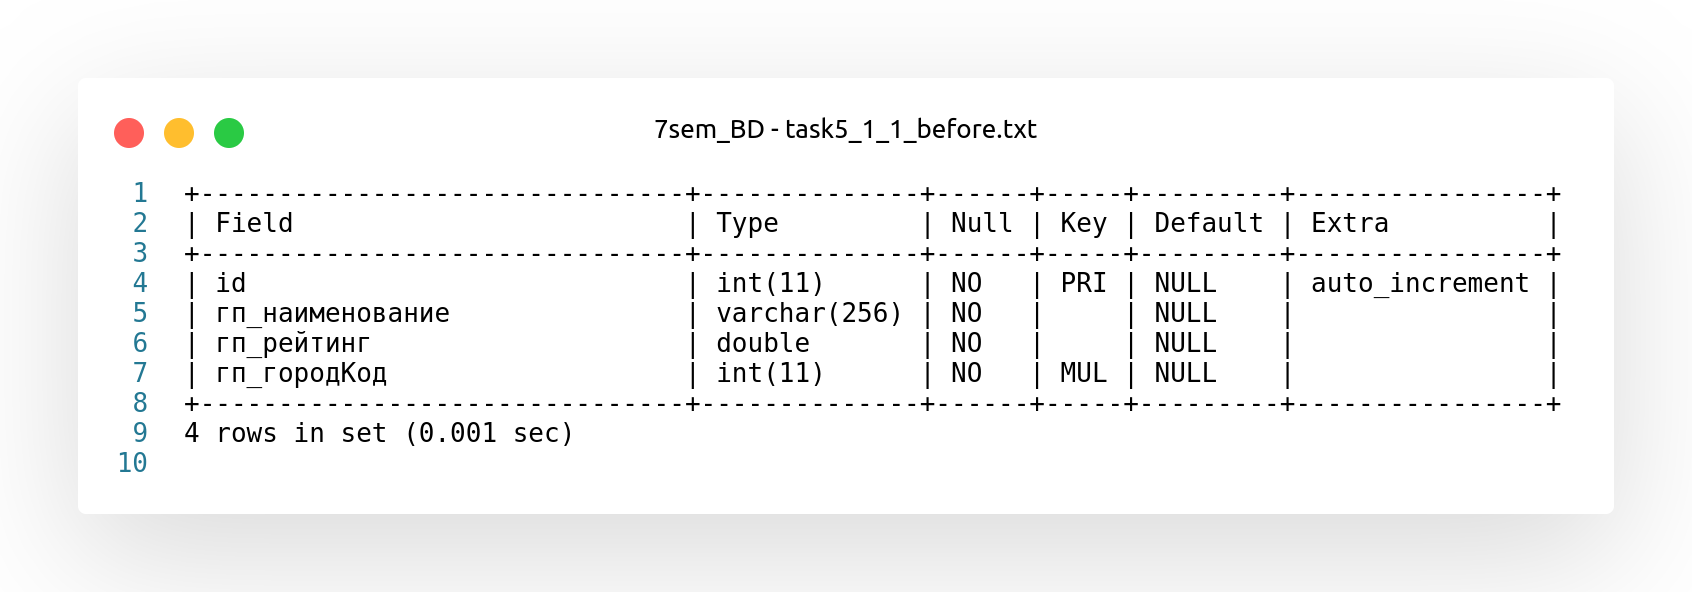
\includegraphics[width=9cm]
    {../sql/task5/task5_1_1_before.png}

    \caption{До ALTER}
    \label{fig:task5_1_1_before}
  \end{minipage}
  \begin{minipage}{0.49\textwidth}
    \centering

    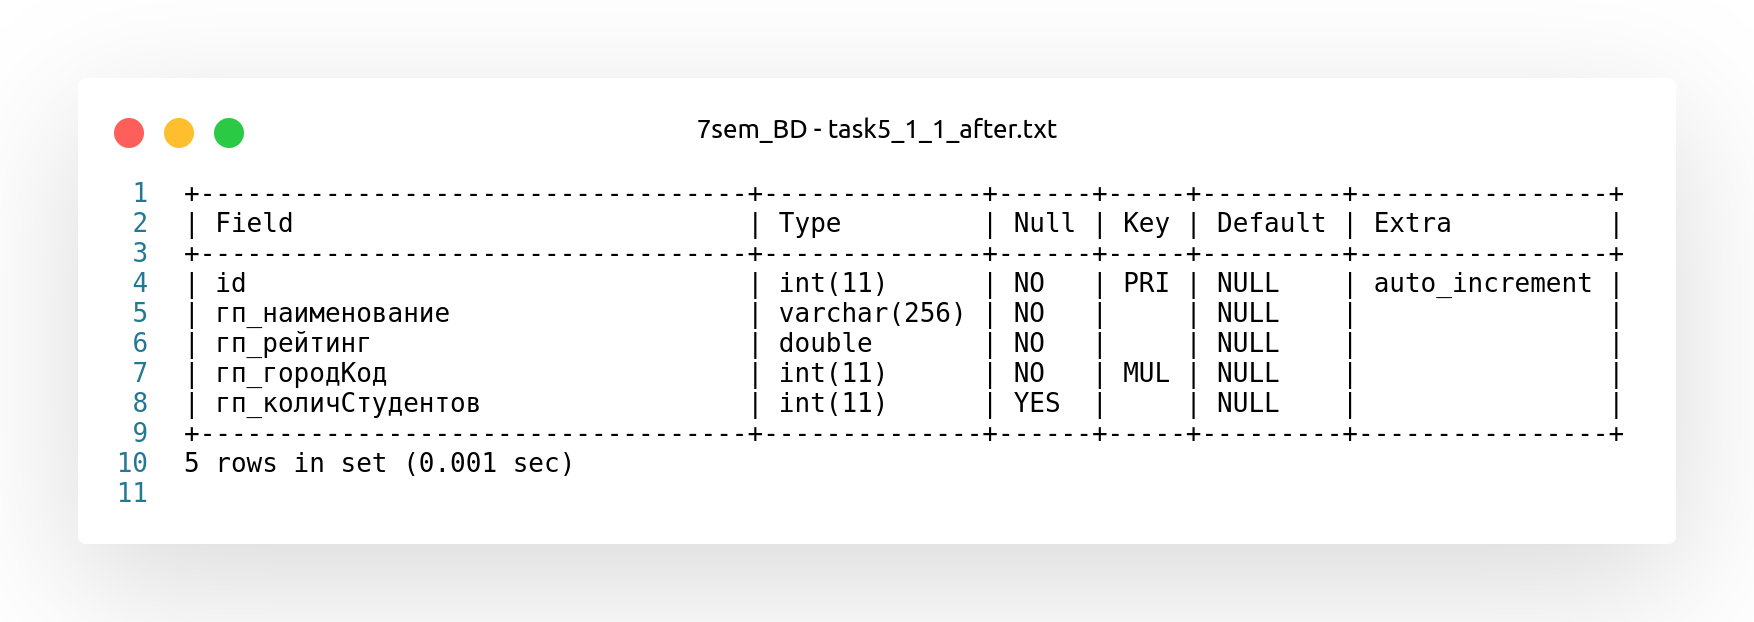
\includegraphics[width=9cm]
    {../sql/task5/task5_1_1_after.png}

    \caption{После ALTER}
    \label{fig:task5_1_1_after}
  \end{minipage}
\end{figure}

\begin{figure}[!h]
  \centering

  \begin{minipage}{0.24\textwidth}
    \centering

    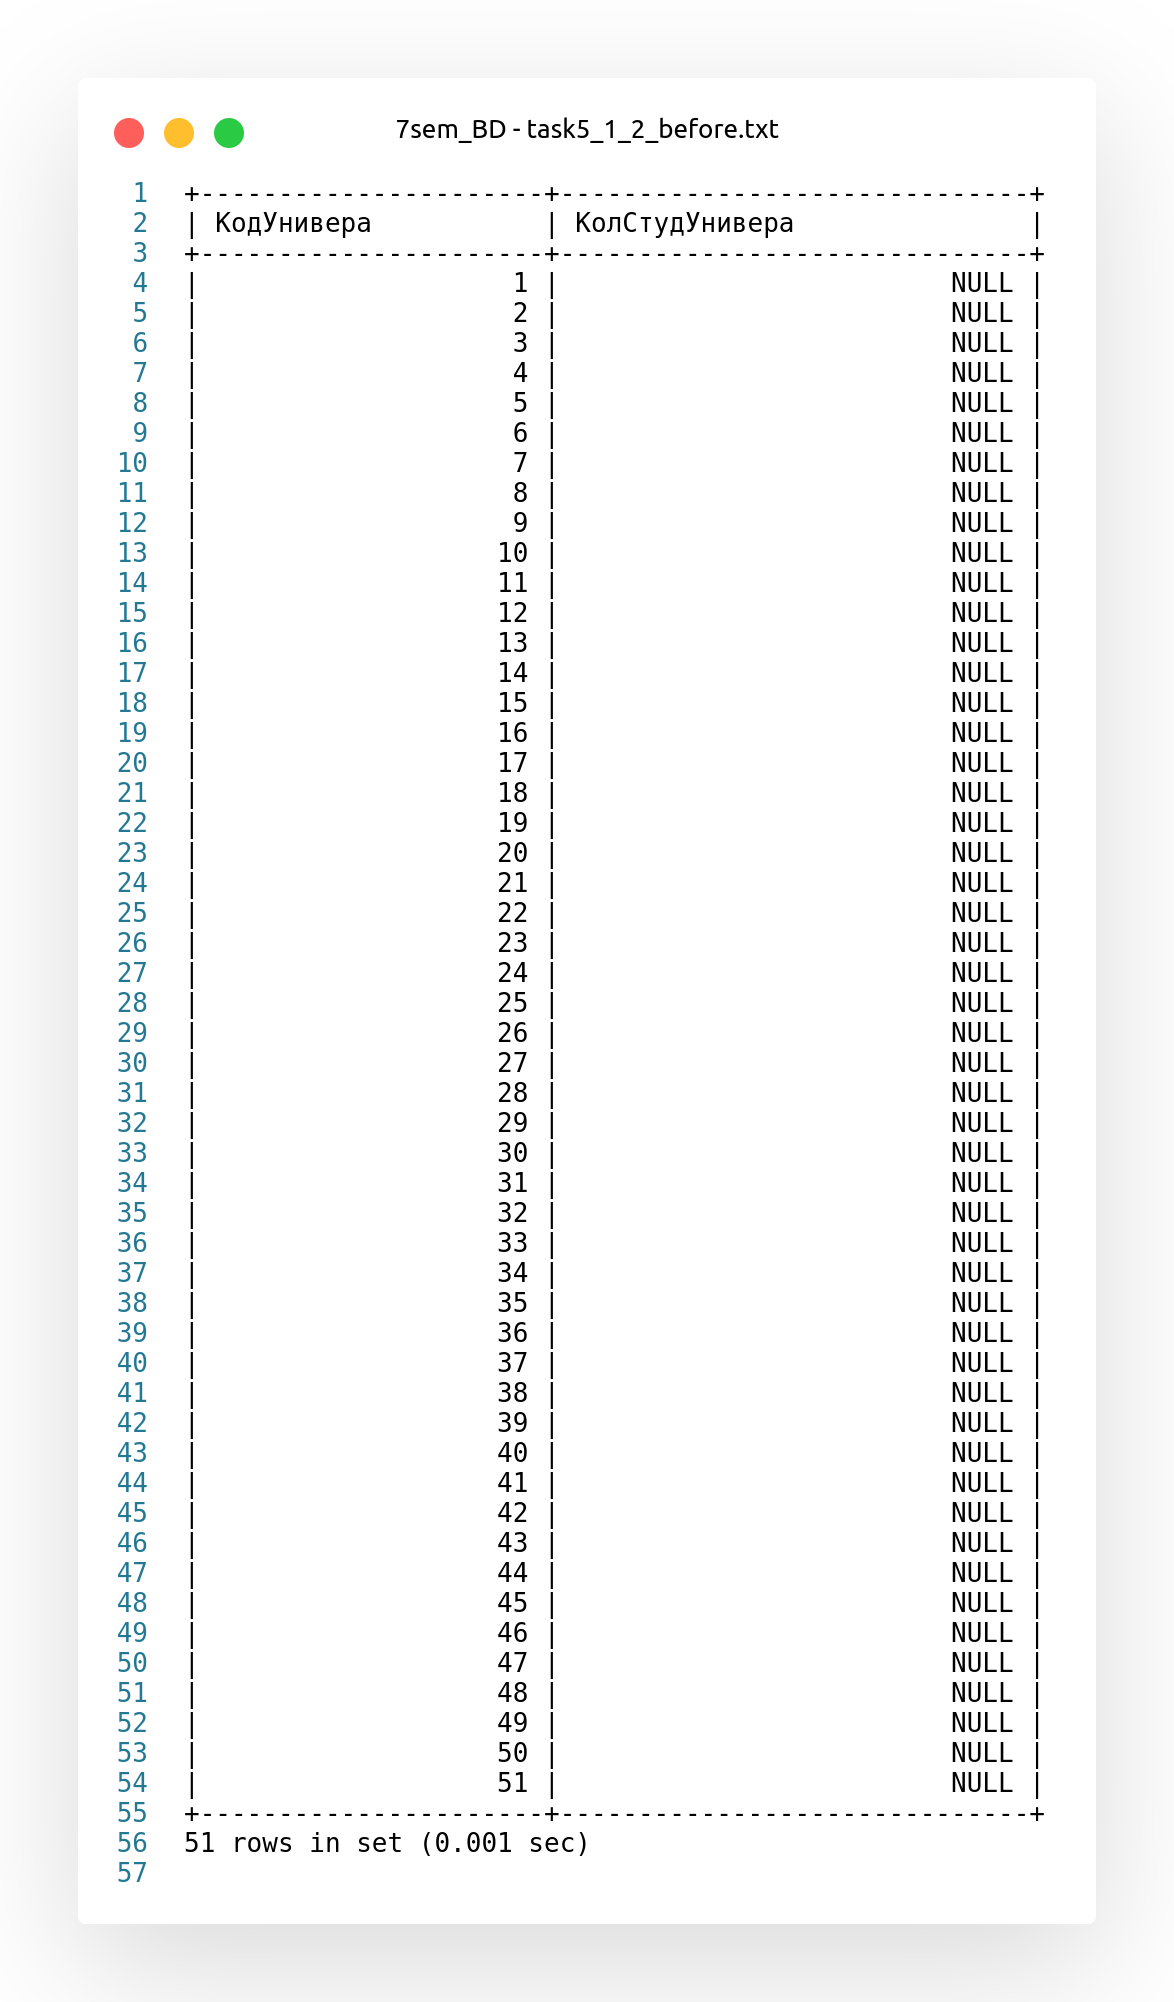
\includegraphics[width=4.5cm]
    {../sql/task5/task5_1_2_before.png}

    \caption{До INSERT}
    \label{fig:task5_1_2_before}
  \end{minipage}
  \begin{minipage}{0.24\textwidth}
    \centering

    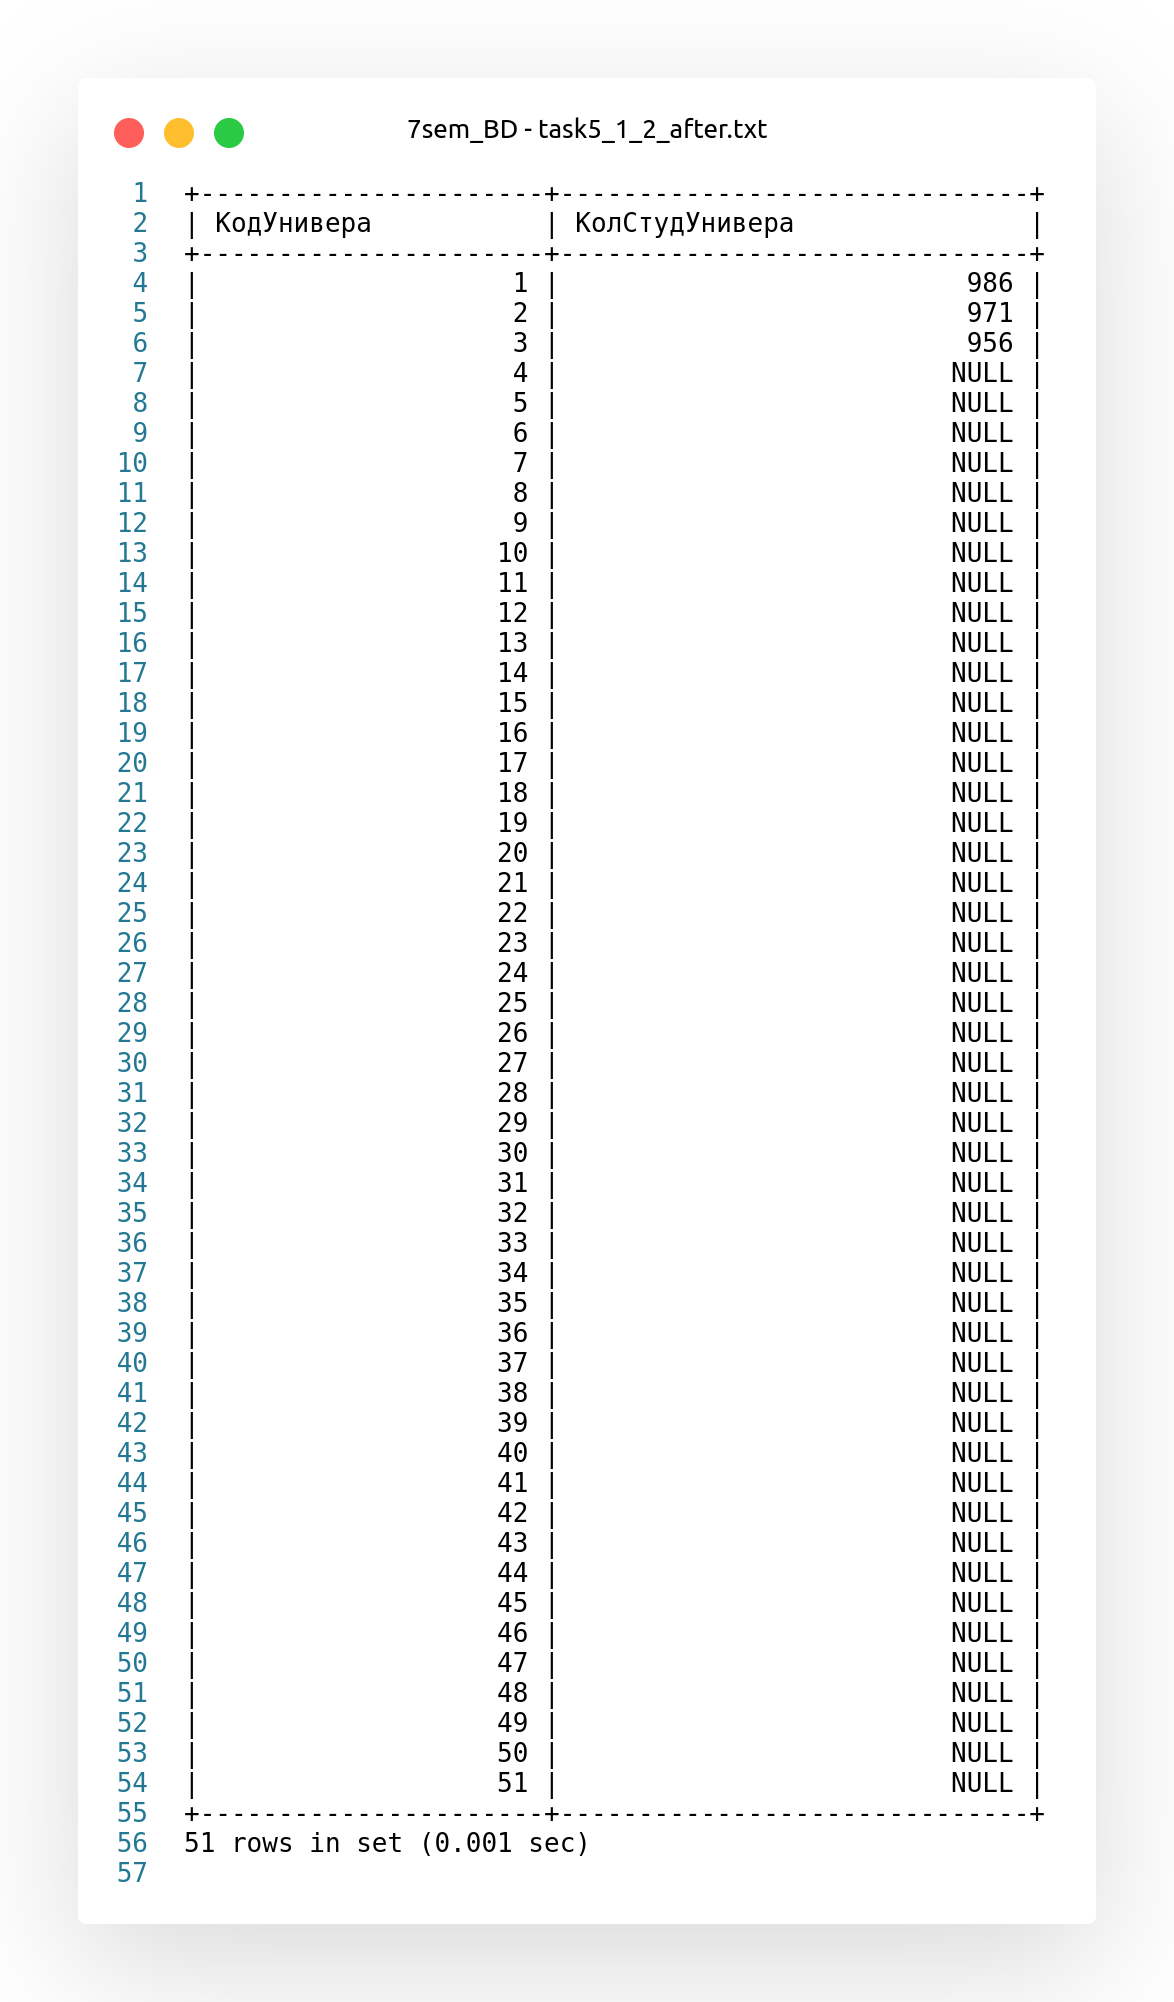
\includegraphics[width=4.5cm]
    {../sql/task5/task5_1_2_after.png}

    \caption{После INSERT}
    \label{fig:task5_1_2_after}
  \end{minipage}
  \begin{minipage}{0.24\textwidth}
    \centering

    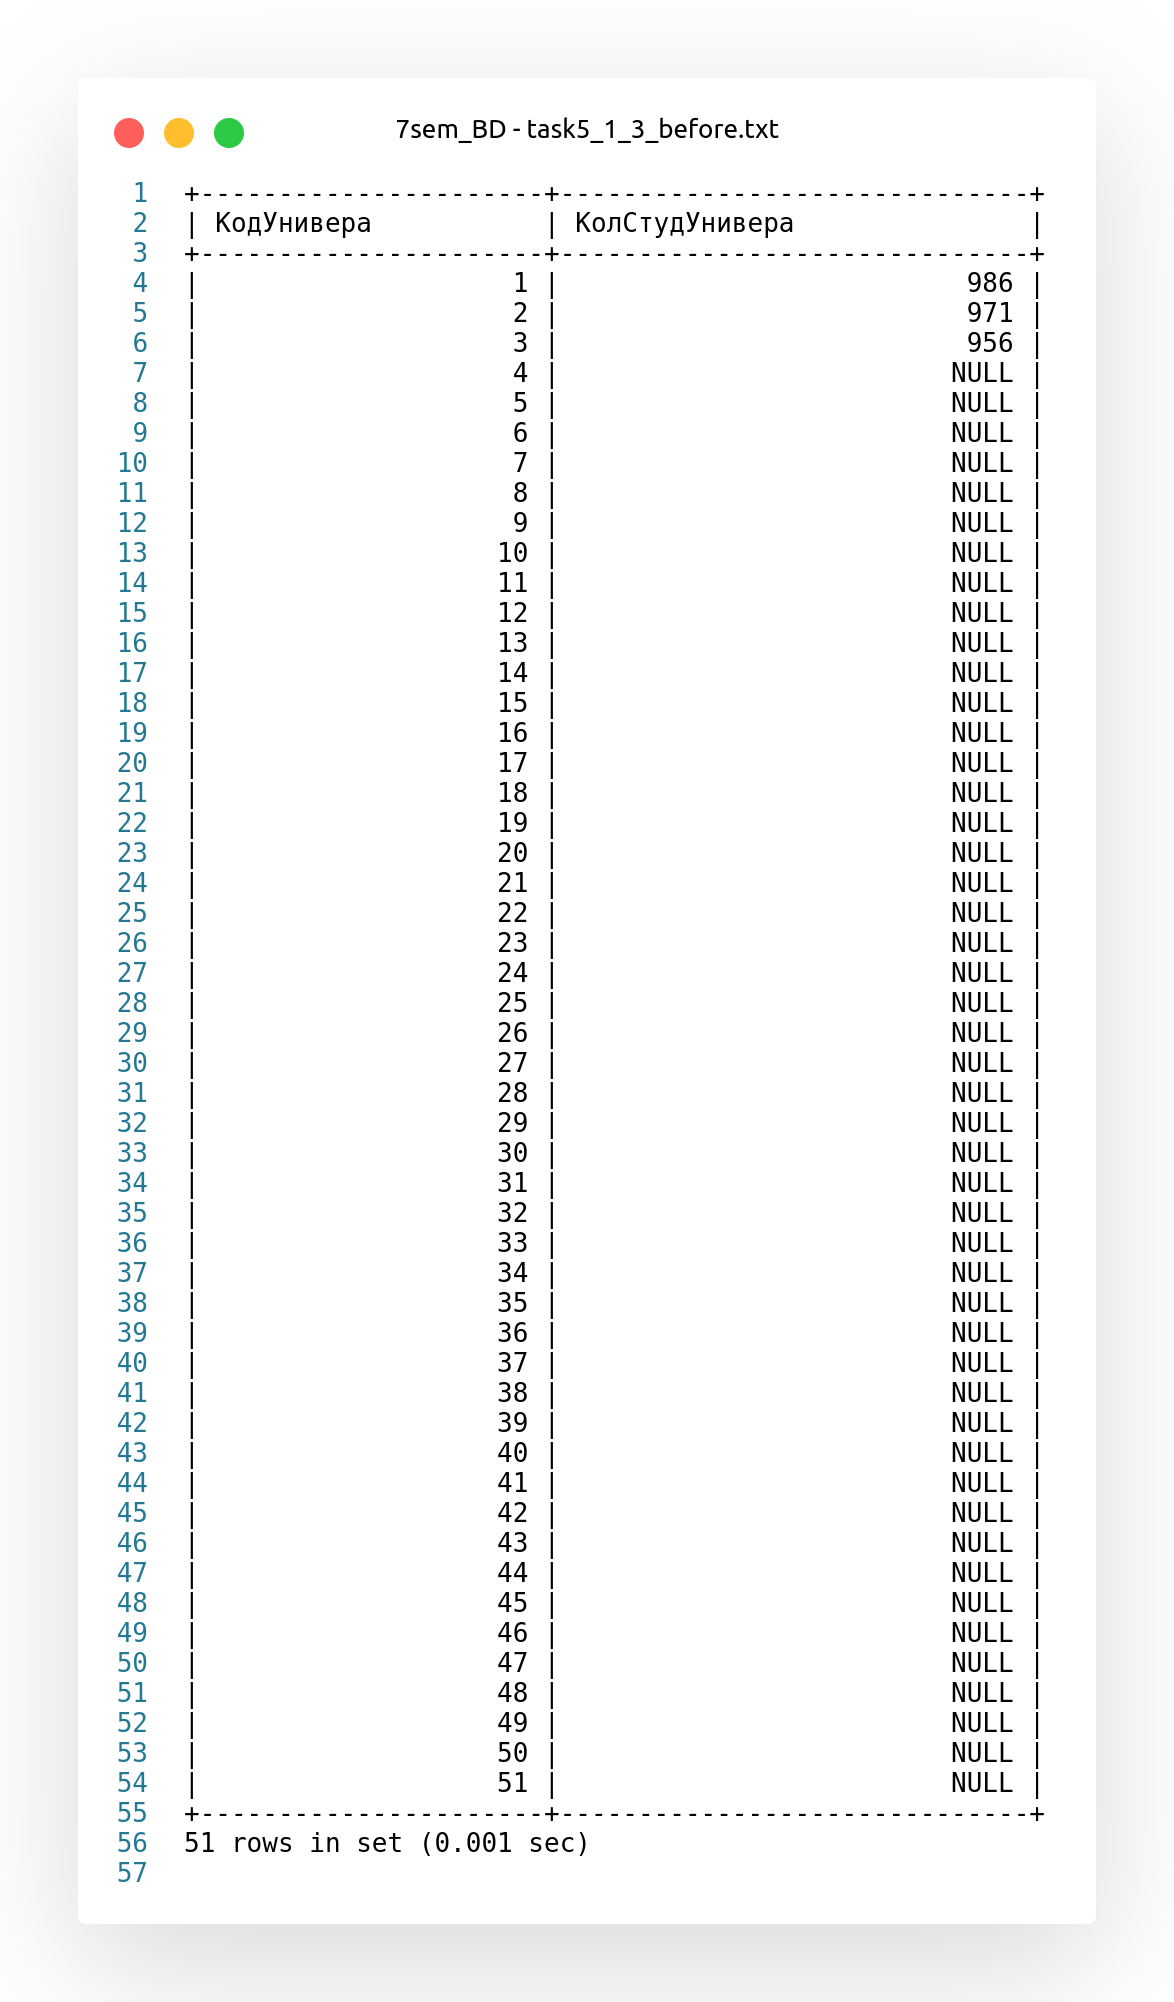
\includegraphics[width=4.5cm]
    {../sql/task5/task5_1_3_before.png}

    \caption{До DELETE}
    \label{fig:task5_1_3_before}
  \end{minipage}
  \begin{minipage}{0.24\textwidth}
    \centering

    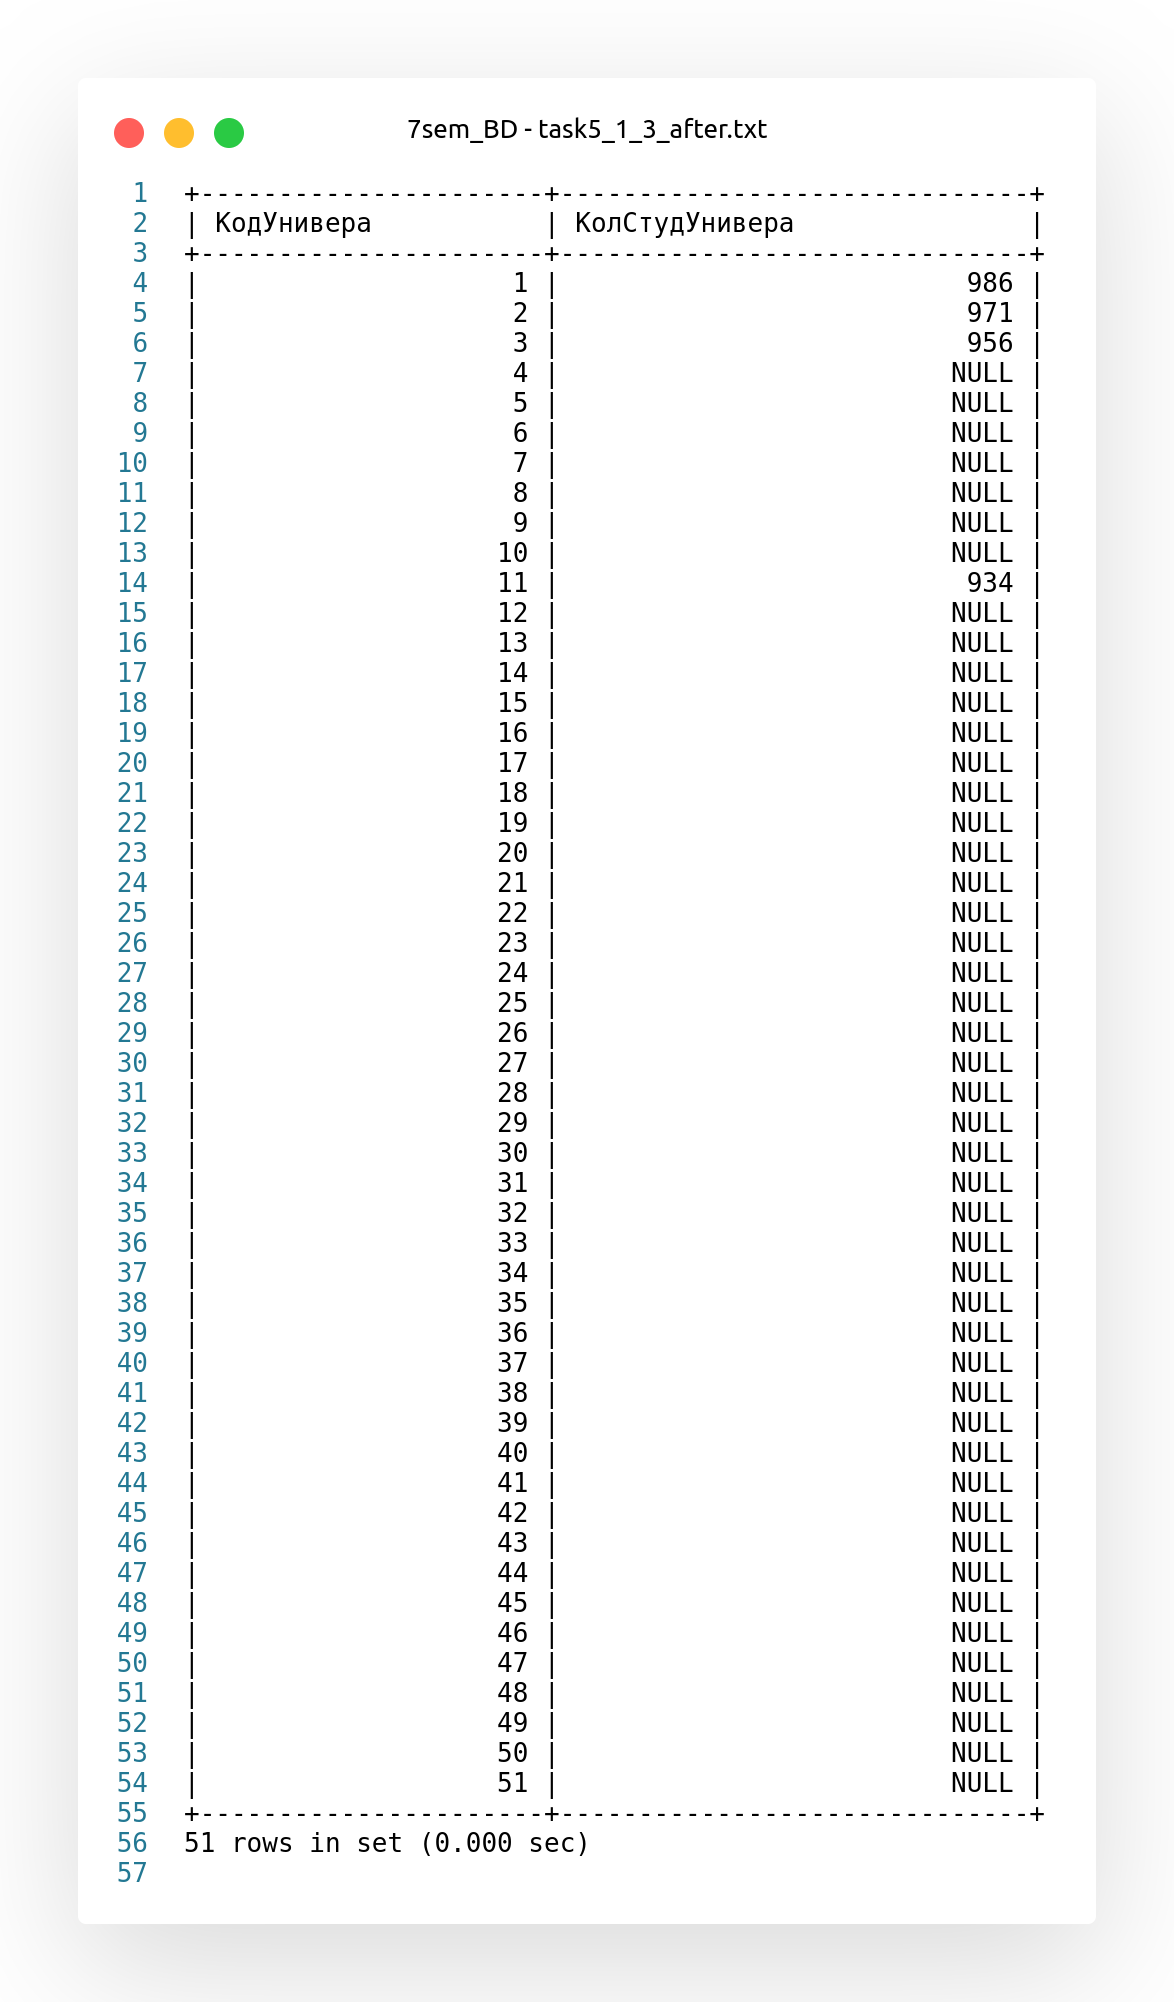
\includegraphics[width=4.5cm]
    {../sql/task5/task5_1_3_after.png}

    \caption{После DELETE}
    \label{fig:task5_1_3_after}
  \end{minipage}
\end{figure}

\begin{center}
  \textbf{Решение задания 5 подпункта 2 (про средний бал универа)}
\end{center}

\lstinputlisting[language=sql]{../sql/task5/task5_2_1.sql}

\lstinputlisting[language=sql]{../sql/task5/task5_2_2.sql}

\lstinputlisting[language=sql]{../sql/task5/task5_2_3.sql}

\lstinputlisting[language=sql]{../sql/task5/task5_2_4.sql}

\textbf{Результаты} изображены
на рисунках~\ref{fig:task5_2_1_before}, \ref{fig:task5_2_1_after},
\ref{fig:task5_2_2_before}, \ref{fig:task5_2_2_after},
\ref{fig:task5_2_3_before}, \ref{fig:task5_2_3_after},
\ref{fig:task5_2_4_before}, \ref{fig:task5_2_4_after}.

\begin{figure}[!h]
  \centering

  \begin{minipage}{0.49\textwidth}
    \centering

    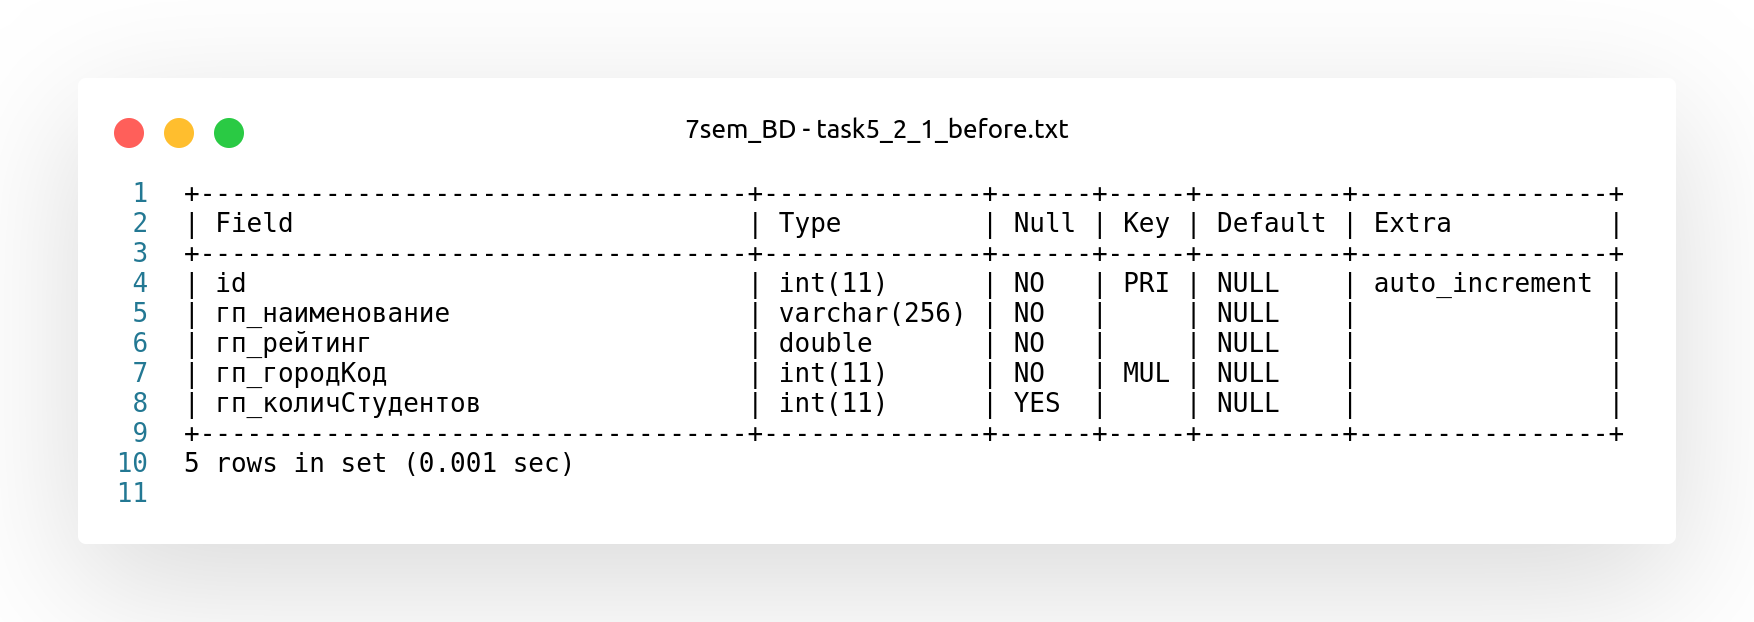
\includegraphics[width=7cm]
    {../sql/task5/task5_2_1_before.png}

    \caption{До ALTER}
    \label{fig:task5_2_1_before}
  \end{minipage}
  \begin{minipage}{0.49\textwidth}
    \centering

    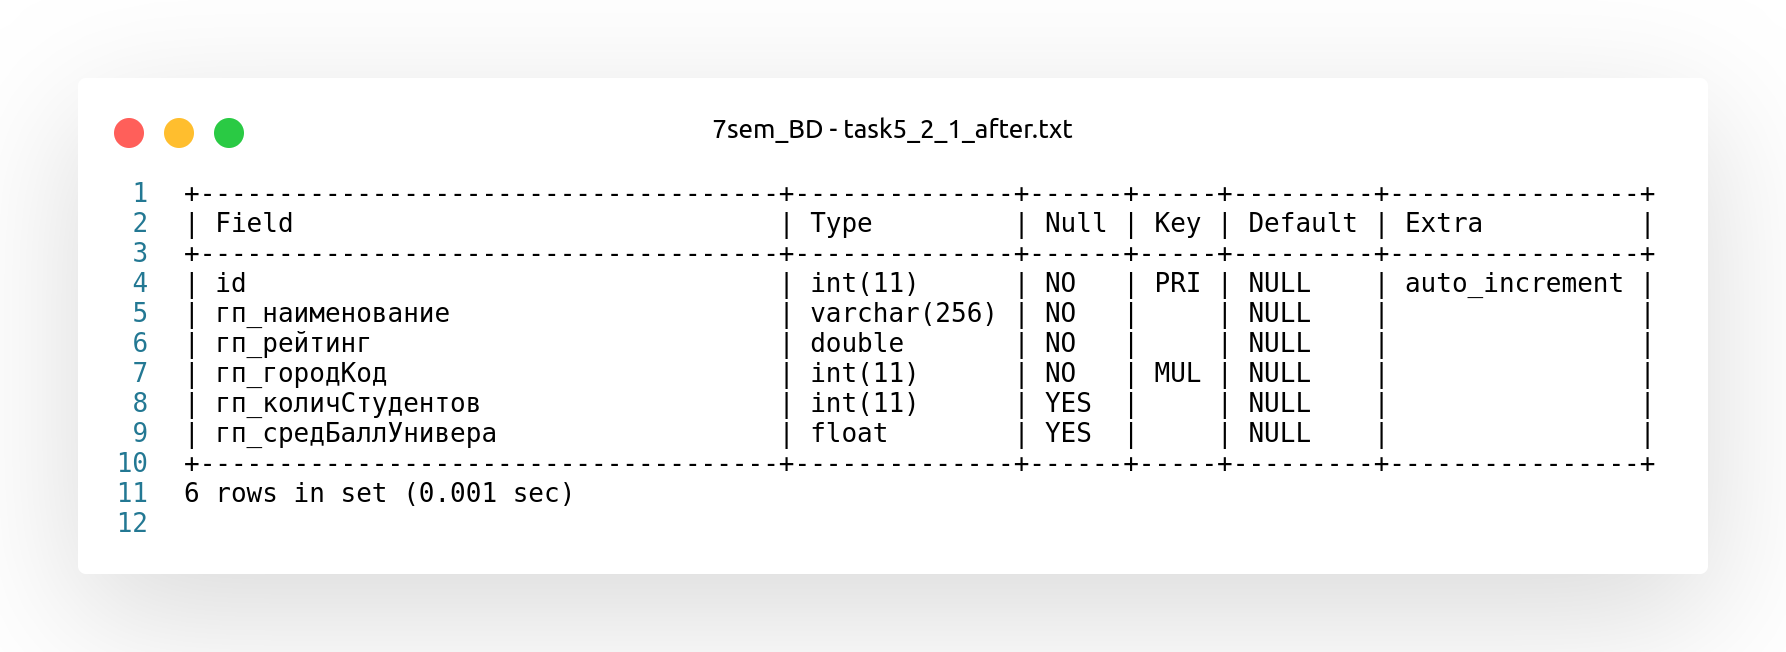
\includegraphics[width=7cm]
    {../sql/task5/task5_2_1_after.png}

    \caption{После ALTER}
    \label{fig:task5_2_1_after}
  \end{minipage}
\end{figure}

\begin{figure}[!h]
  \centering

  \begin{minipage}{0.24\textwidth}
    \centering

    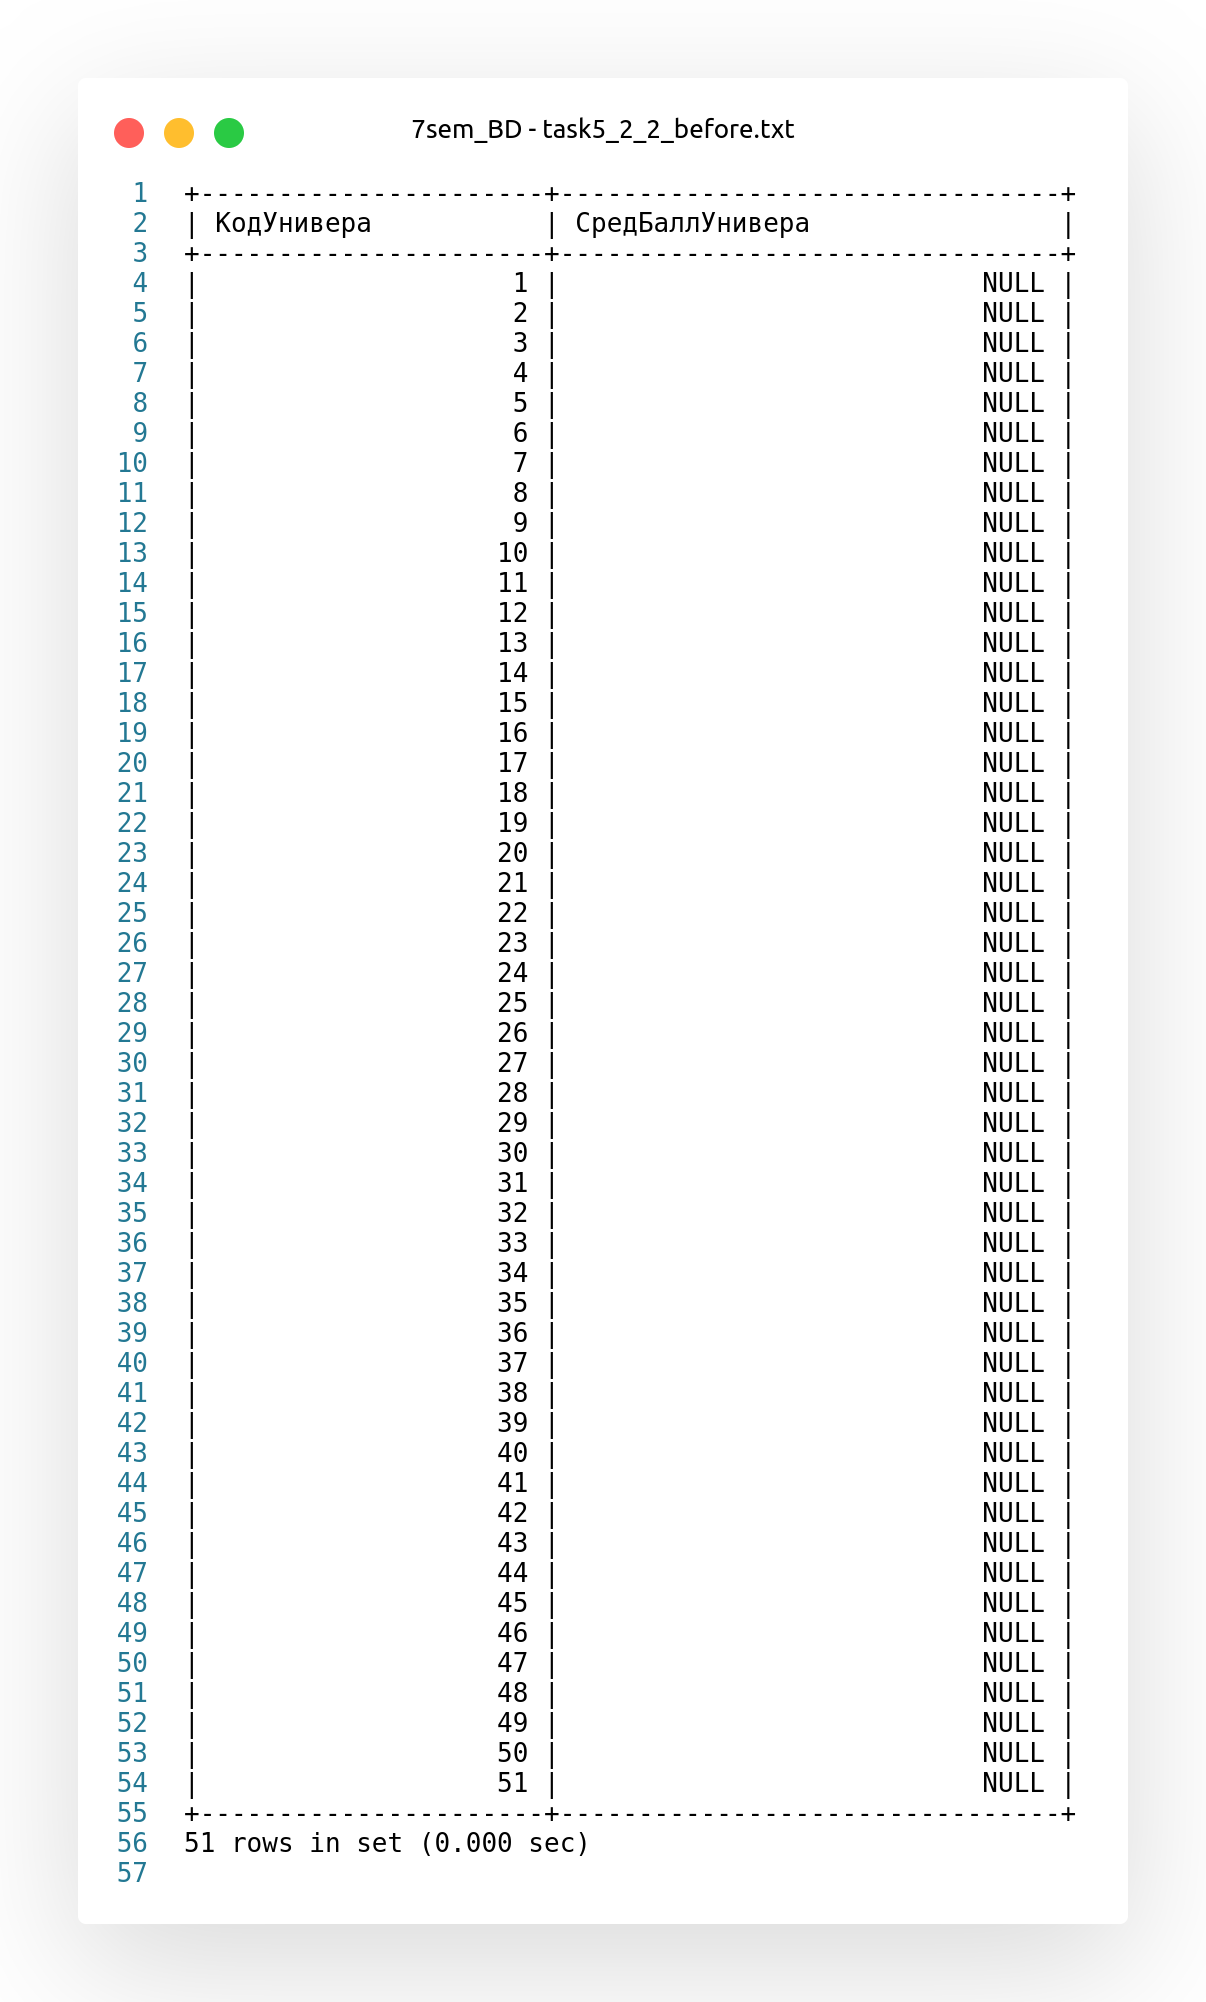
\includegraphics[width=4.5cm]
    {../sql/task5/task5_2_2_before.png}

    \caption{До INSERT}
    \label{fig:task5_2_2_before}
  \end{minipage}
  \begin{minipage}{0.24\textwidth}
    \centering

    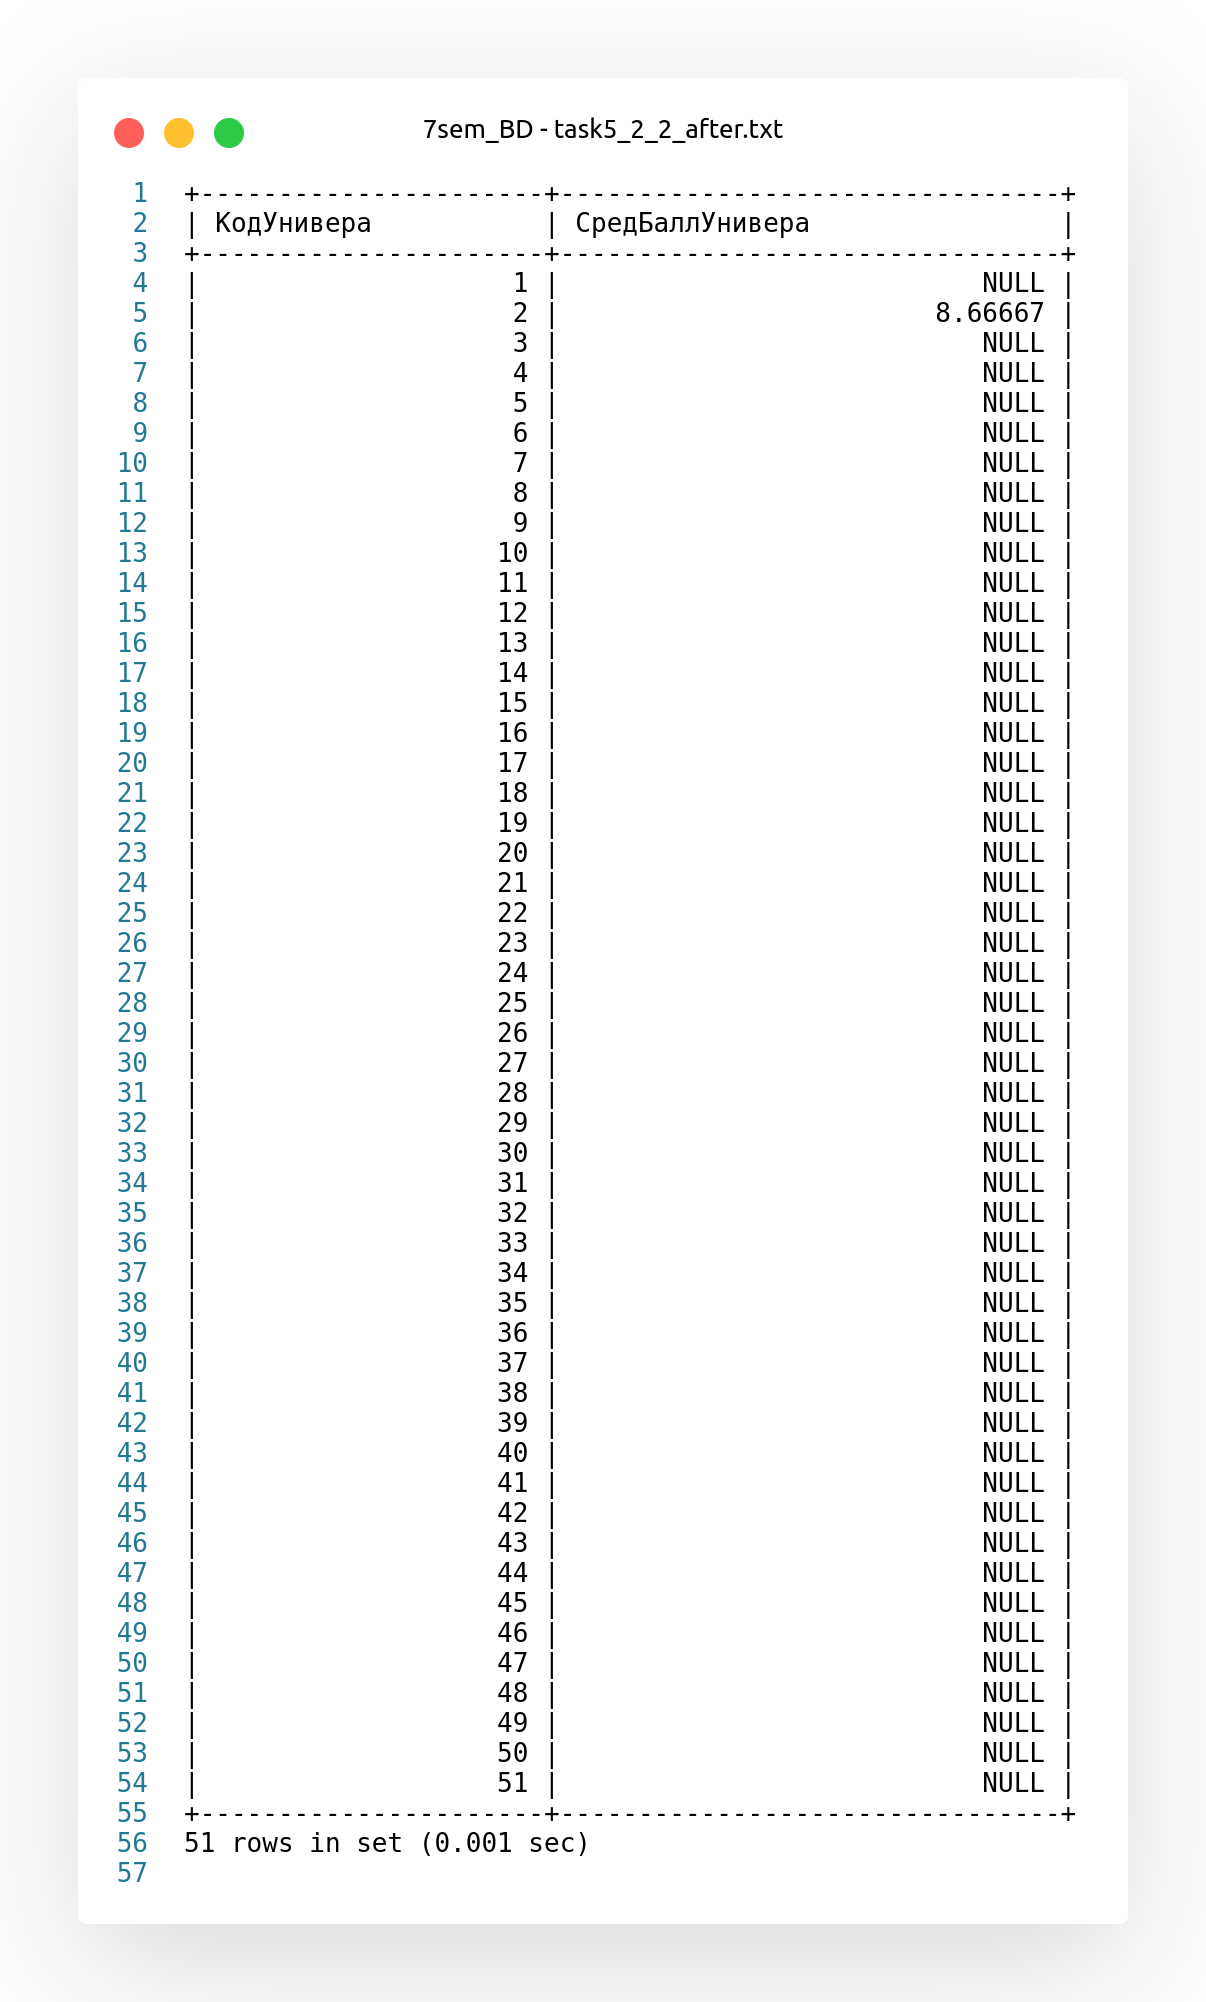
\includegraphics[width=4.5cm]
    {../sql/task5/task5_2_2_after.png}

    \caption{После INSERT}
    \label{fig:task5_2_2_after}
  \end{minipage}
  \begin{minipage}{0.24\textwidth}
    \centering

    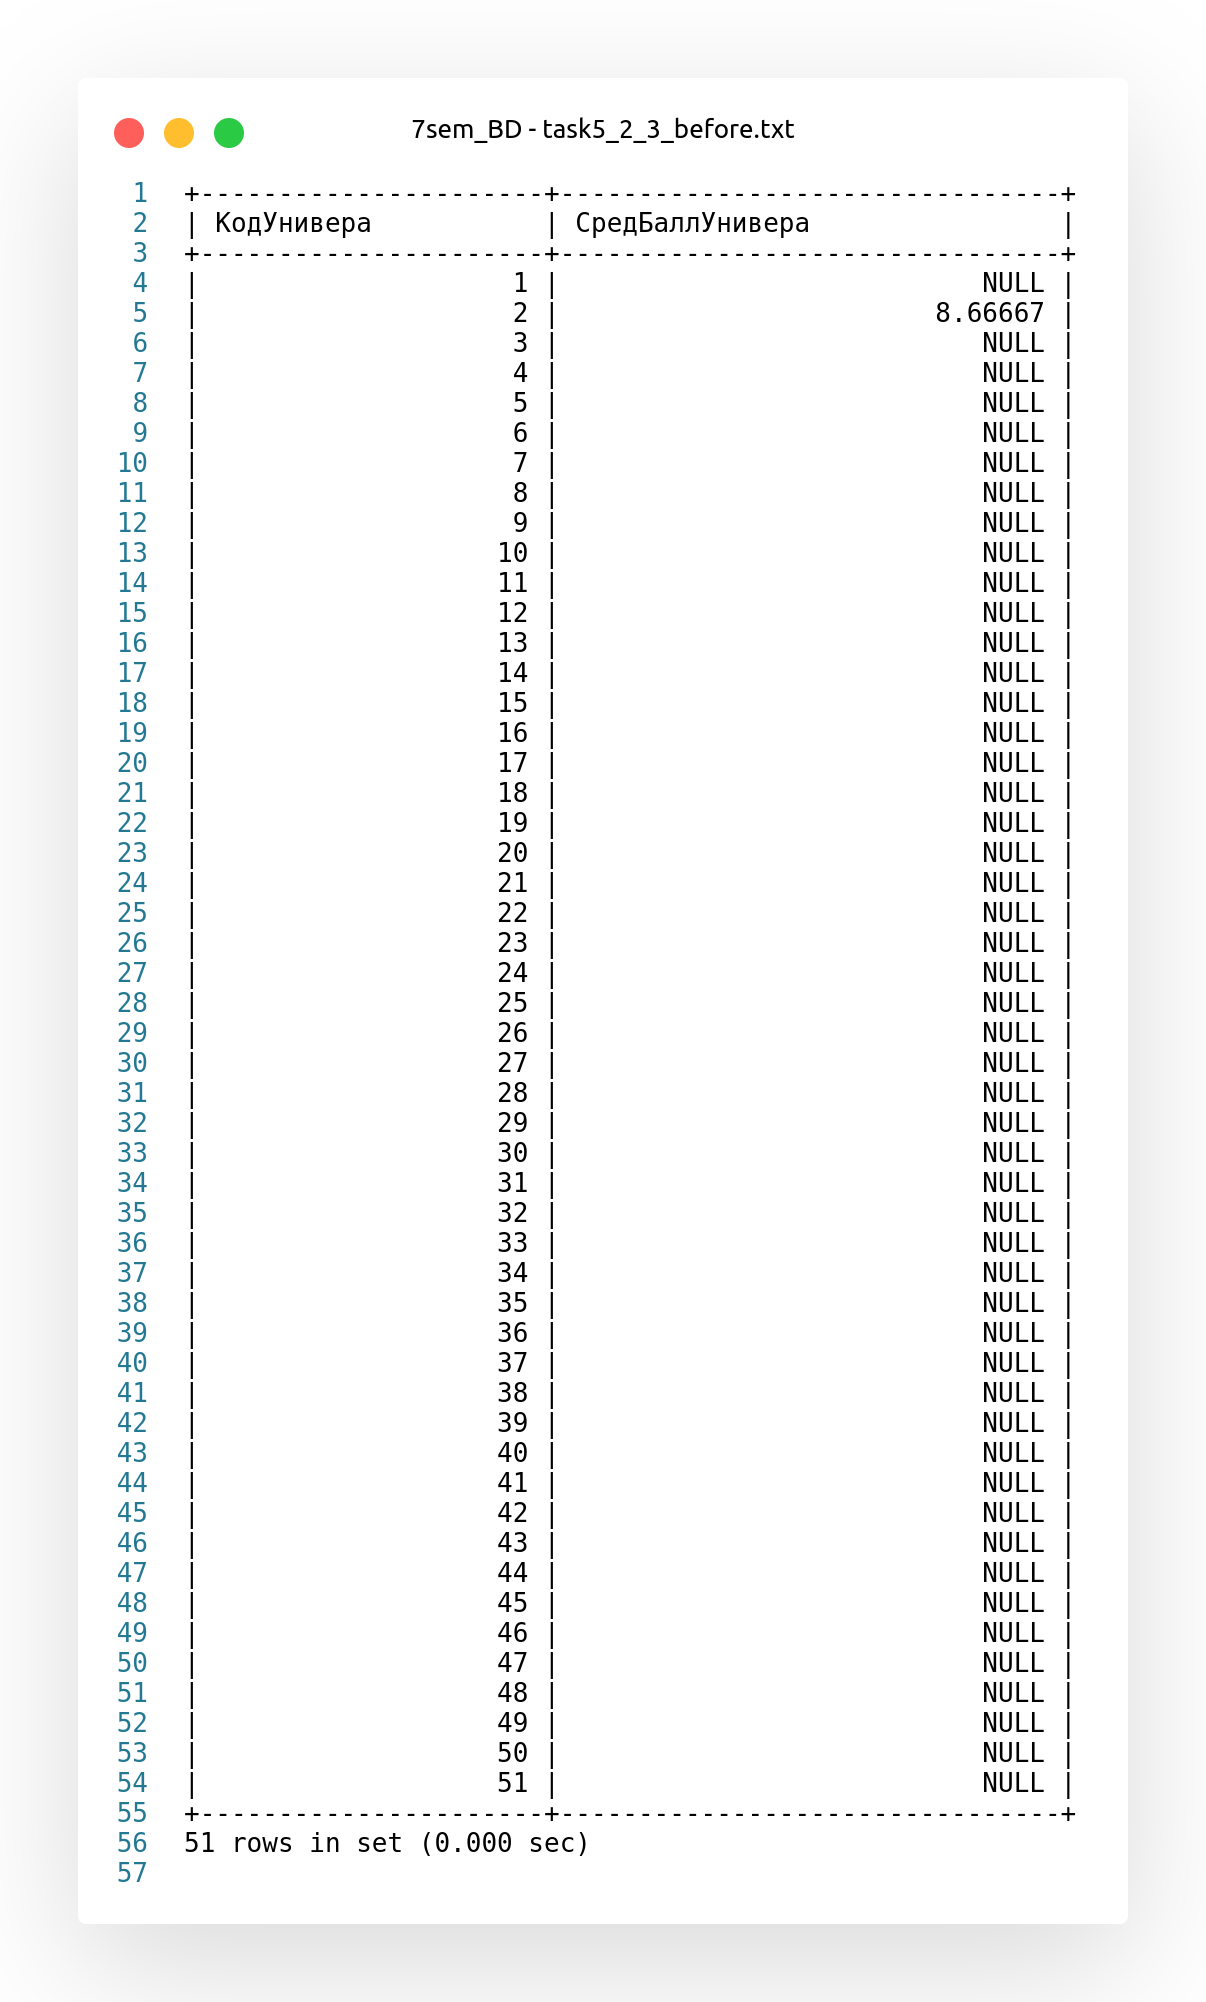
\includegraphics[width=4.5cm]
    {../sql/task5/task5_2_3_before.png}

    \caption{До DELETE}
    \label{fig:task5_2_3_before}
  \end{minipage}
  \begin{minipage}{0.24\textwidth}
    \centering

    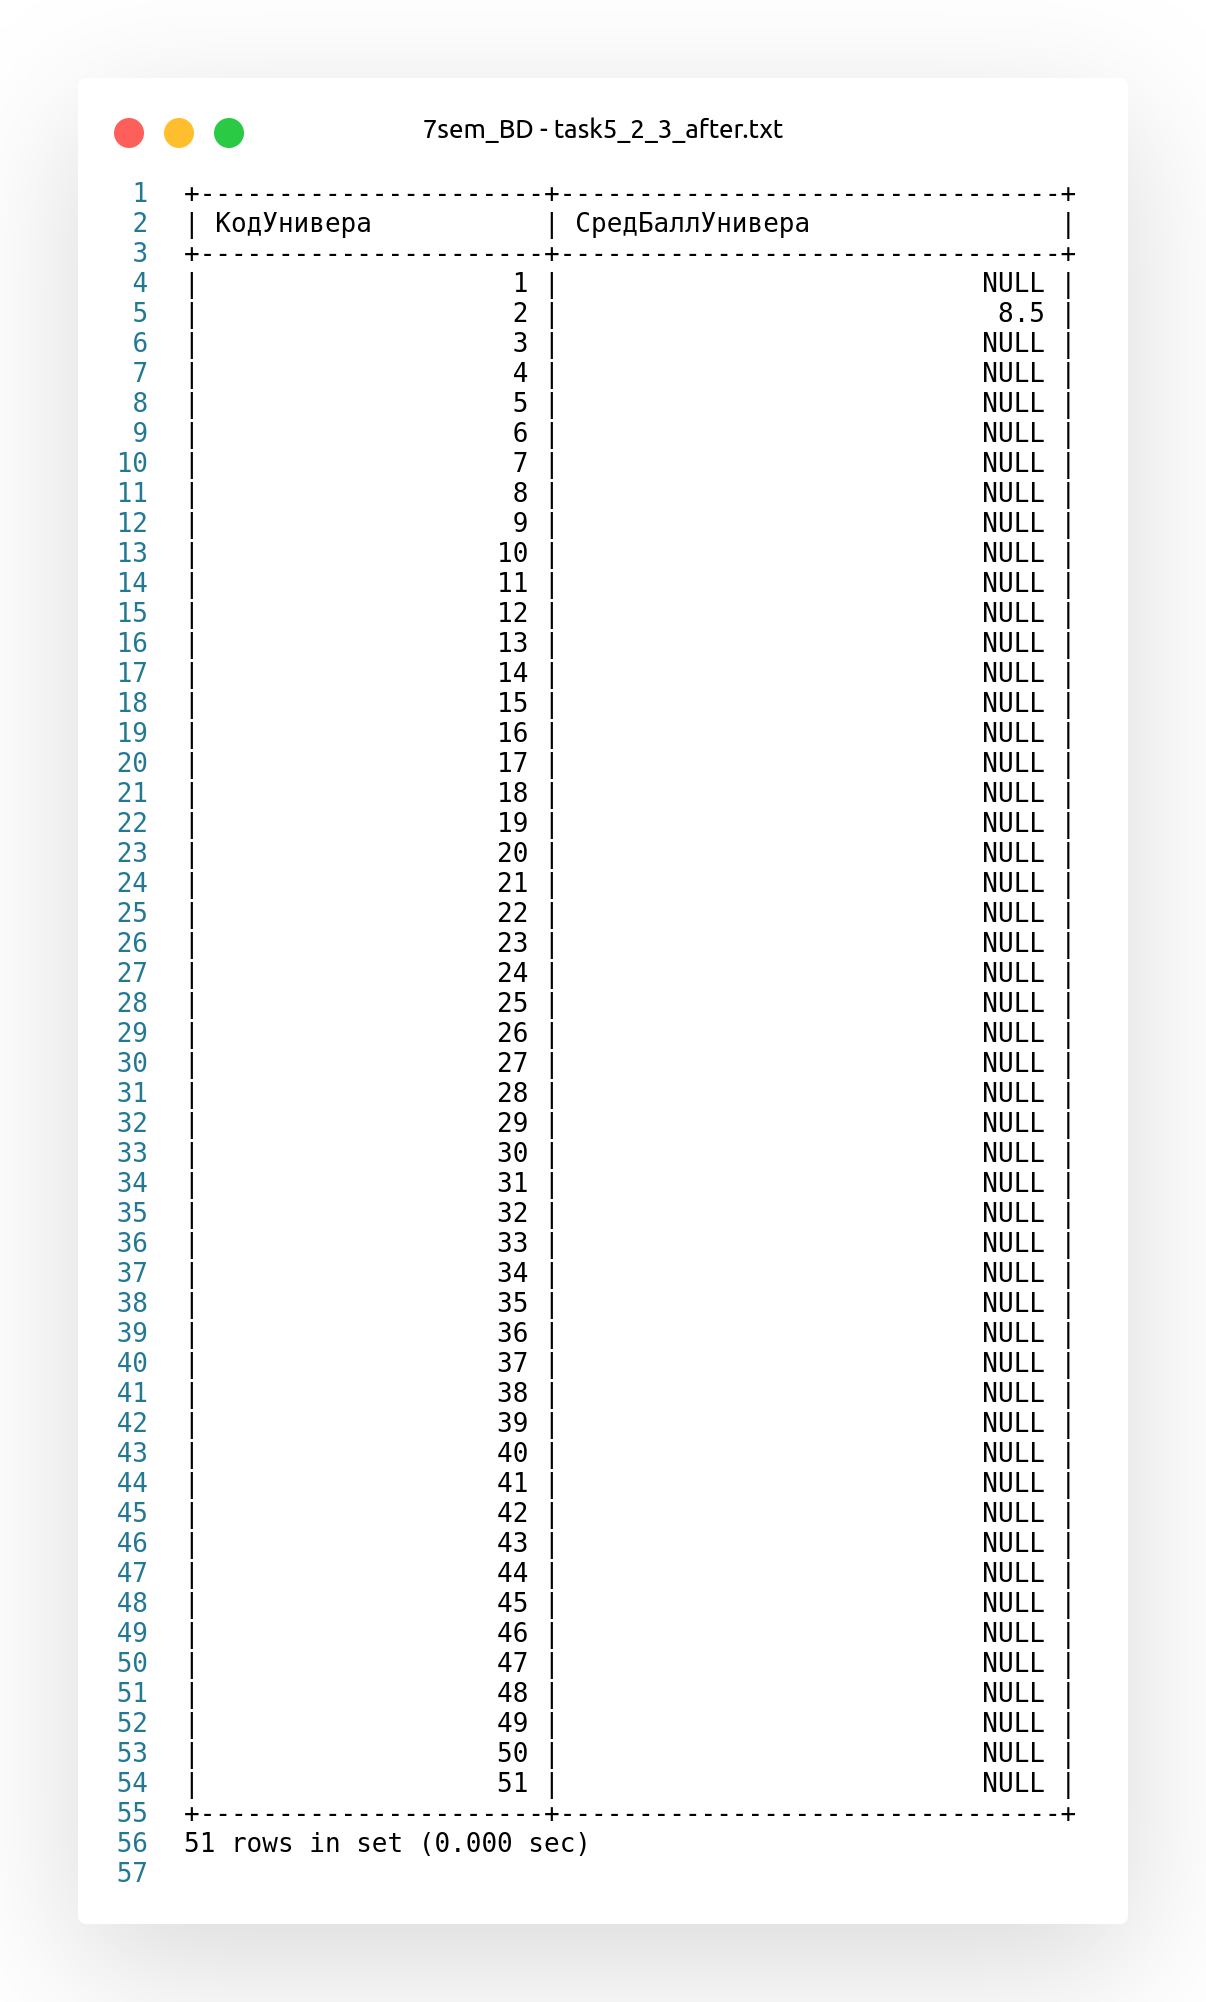
\includegraphics[width=4.5cm]
    {../sql/task5/task5_2_3_after.png}

    \caption{После DELETE}
    \label{fig:task5_2_3_after}
  \end{minipage}
\end{figure}

\begin{figure}[!h]
  \centering

  \begin{minipage}{0.49\textwidth}
    \centering

    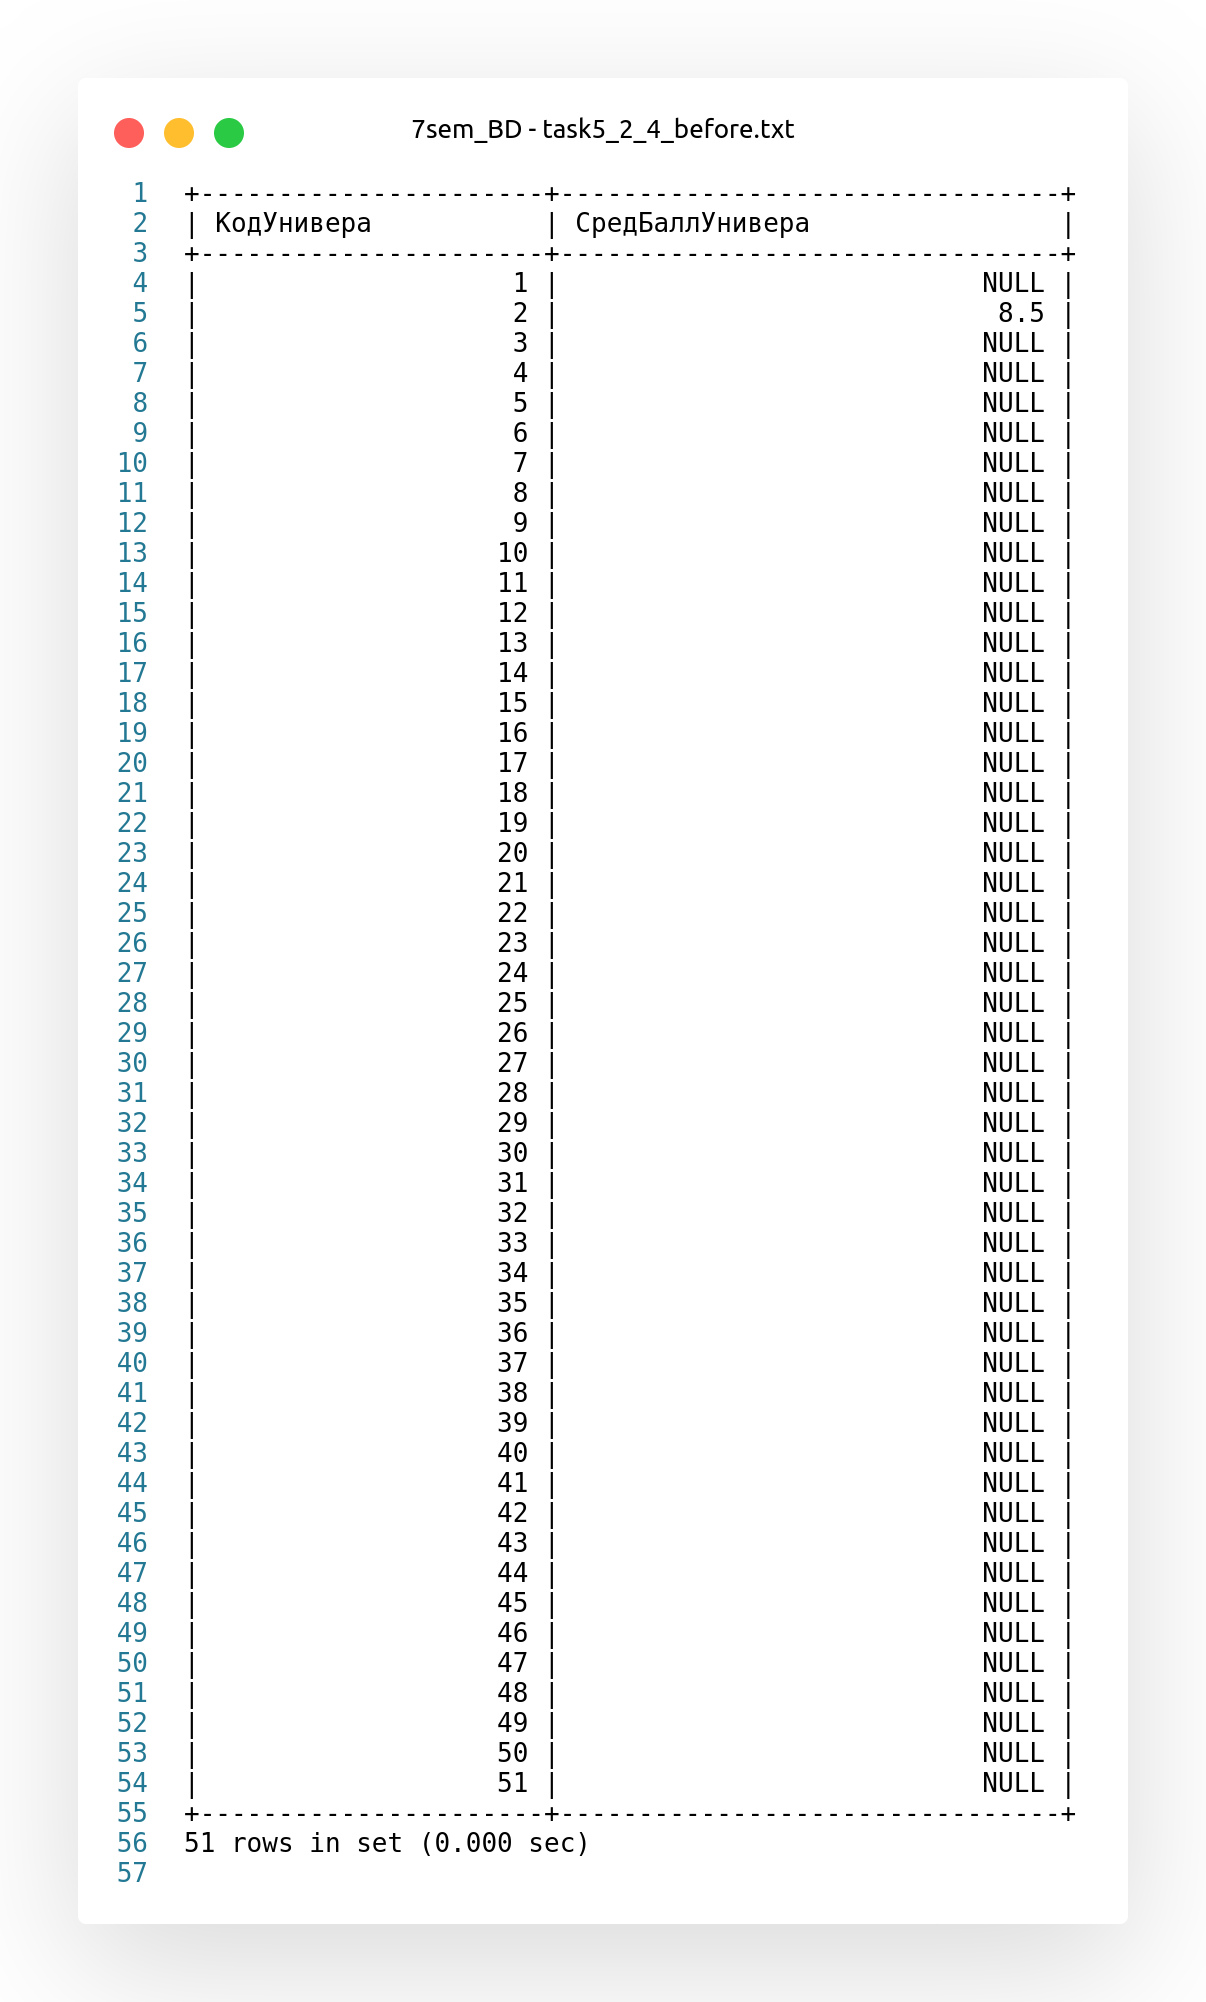
\includegraphics[width=4.5cm]
    {../sql/task5/task5_2_4_before.png}

    \caption{До UPDATE}
    \label{fig:task5_2_4_before}
  \end{minipage}
  \begin{minipage}{0.49\textwidth}
    \centering

    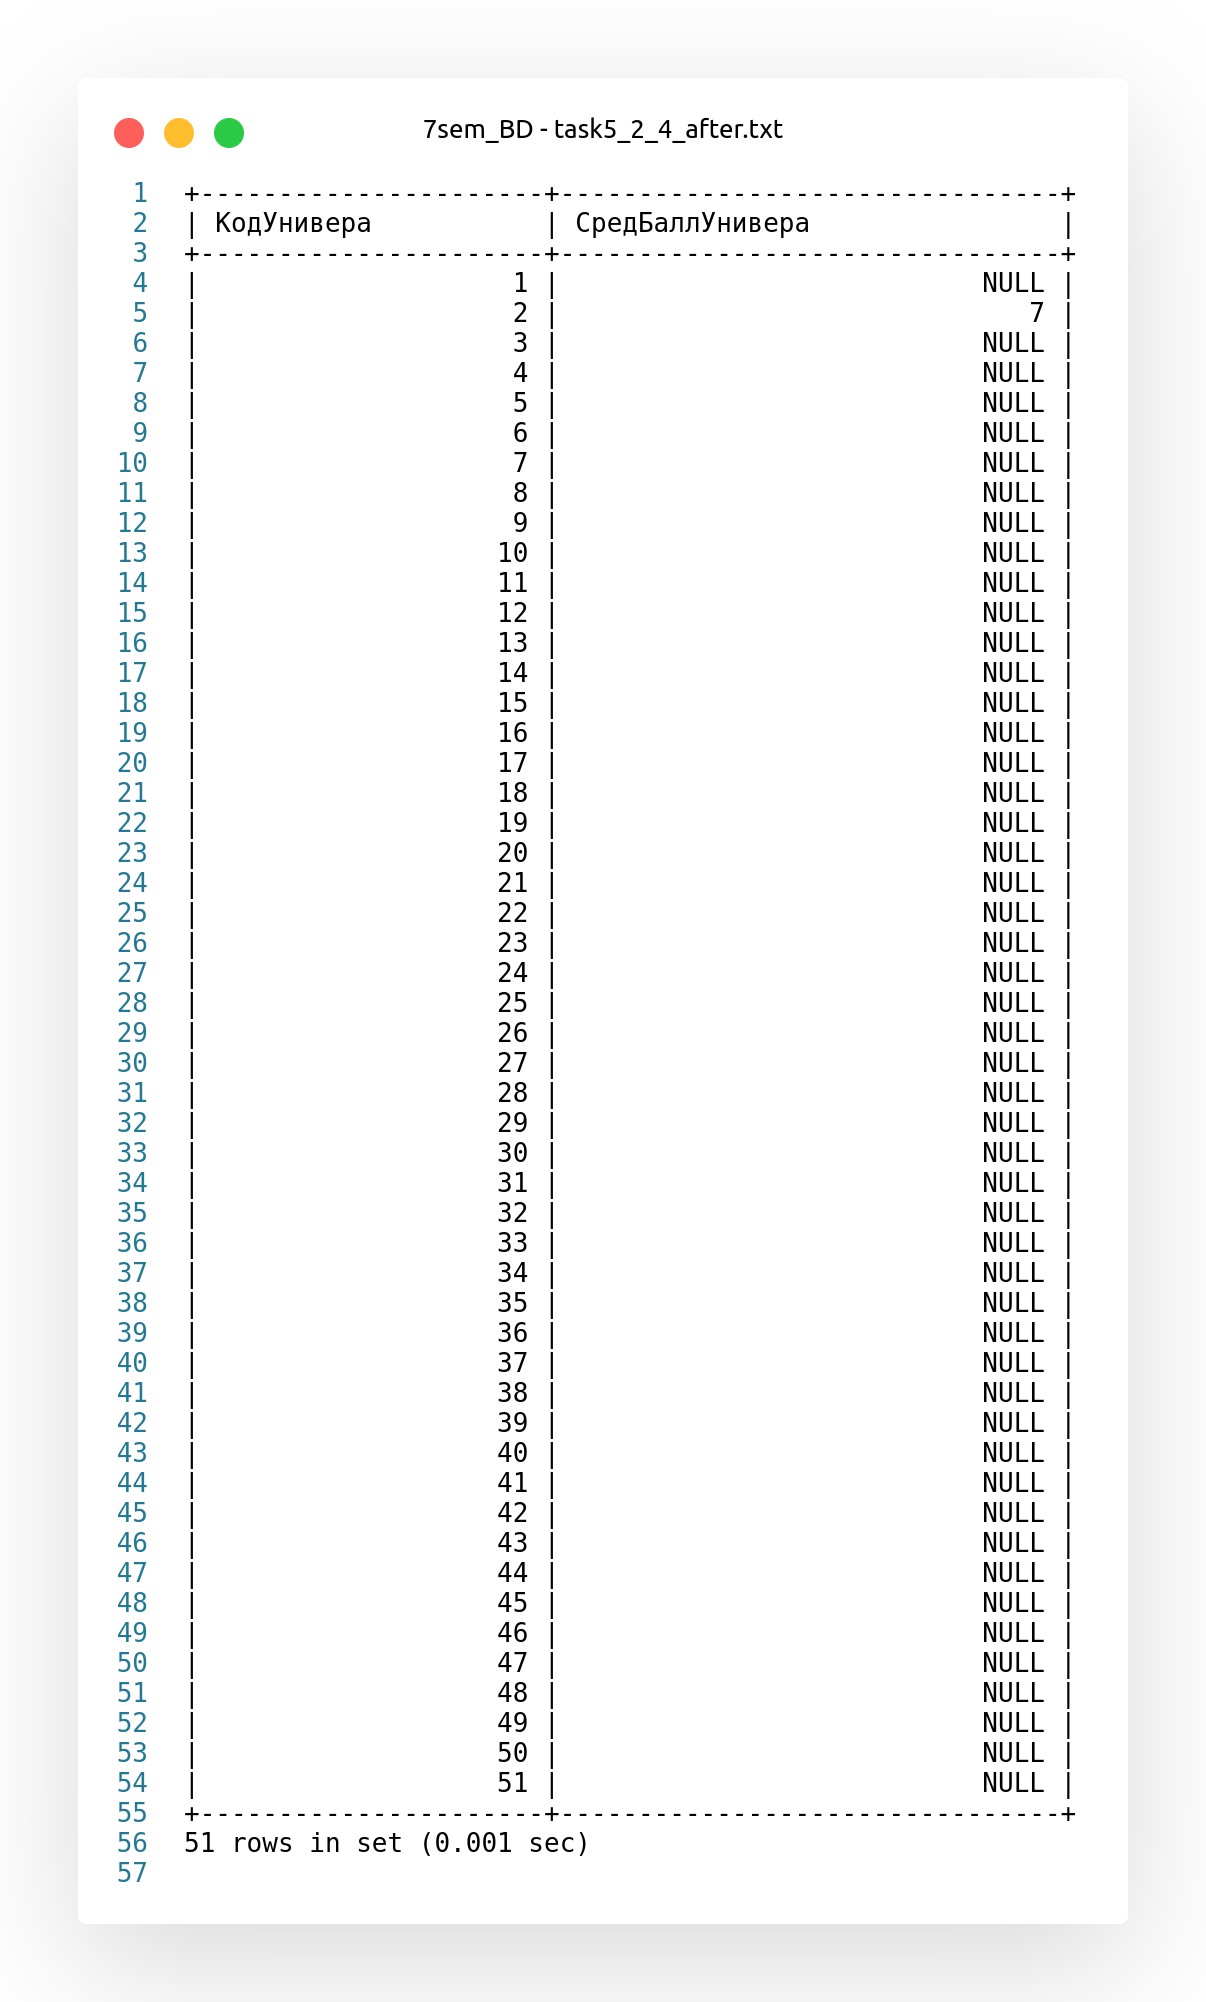
\includegraphics[width=4.5cm]
    {../sql/task5/task5_2_4_after.png}

    \caption{После UPDATE}
    \label{fig:task5_2_4_after}
  \end{minipage}
\end{figure}

\newpage

\begin{center}
  \textbf{Решение задания 5 подпункта 4 (про комментарии о рейтинге универа)}
\end{center}

\lstinputlisting[language=sql]{../sql/task5/task5_4_1.sql}

\lstinputlisting[language=sql]{../sql/task5/task5_4_2.sql}
